% !TeX program = xelatex
\documentclass[a4paper, 12pt]{report}
% Biên dịch bằng XeLaTeX để hỗ trợ tiếng Việt Unicode.
\usepackage{fontspec}
\setmainfont{TeX Gyre Termes}
\usepackage{polyglossia}
\setmainlanguage{vietnamese}
\setotherlanguage{english}
\usepackage{graphicx}
\usepackage{geometry}
\usepackage{tocloft,calc}
\usepackage{amsmath,amsfonts,latexsym}
\usepackage{fancyhdr}
\usepackage{tikz}
\usepackage{eso-pic}
\usepackage{indentfirst}
\usepackage{setspace}
\usepackage[unicode,bookmarks=true,colorlinks=true]{hyperref}
\usepackage[capitalize]{cleveref}
% cleveref chưa có bộ tên ngôn ngữ Vietnamese; dùng hook tiếng Anh của nó,
% còn nhãn tham chiếu tiếng Việt được đặt ngay bên dưới.
\makeatletter
\def\cref@language{english}
\makeatother
\crefname{figure}{Hình}{Hình}
\Crefname{figure}{Hình}{Hình}
\crefname{table}{Bảng}{Bảng}
\Crefname{table}{Bảng}{Bảng}
\crefname{chapter}{Chương}{Chương}
\Crefname{chapter}{Chương}{Chương}
\usepackage{booktabs}
\usepackage{algorithm}
\usepackage{algpseudocode}
\floatname{algorithm}{Thuật toán}
\algrenewcommand\algorithmicrequire{\textbf{Đầu vào:}}
\algrenewcommand\algorithmicensure{\textbf{Đầu ra:}}
\usepackage{tabularx}
\usepackage{longtable}
\usepackage{multirow}
\usepackage[official]{eurosym}   % biểu tượng euro
\usepackage{enumitem}
\usepackage[table]{xcolor}
\usepackage{float}
\usepackage{chngcntr}
\usepackage[version=4]{mhchem}
\usepackage{fancybox}
\counterwithout{figure}{chapter}

\hypersetup{
  pdftitle={Khảo sát giải mã suy đoán không sử dụng bộ nhớ trọng số bổ sung trên GPU giới hạn tài nguyên},
  pdfauthor={Nguyễn Quốc Hiếu},
  linkcolor=blue,
  citecolor=blue,
  urlcolor=blue
}

\onehalfspacing

\geometry{
    top=3.5cm, 
    bottom=3.0cm, 
    left=3.5cm, 
    right=2.0cm
  % left=64pt,
  % right=64pt,
  % top=64pt,
  % bottom=64pt,
}

\usetikzlibrary{calc}

\newcommand{\drawcoverframe}{
    \AddToShipoutPicture*{%
    \begin{tikzpicture}[remember picture,overlay]
        % Khung ngoài
        \draw[line width=2pt]
            ($(current page.north west)+(3.5cm,-3.5cm)$)
            rectangle
            ($(current page.south east)+(-2cm,3cm)$);
    
        % Khung trong
        \draw[line width=1pt]
            ($(current page.north west)+(3.65cm,-3.65cm)$)
            rectangle
            ($(current page.south east)+(-2.15cm,3.15cm)$);
    \end{tikzpicture}
    }
}

\setlength{\headheight}{16pt}
\pagestyle{fancy}
\fancyhf{}
\lhead{}
\rhead{}
\cfoot{\thepage}

% Hide the printed "Chương <n>" heading label, but keep chapter numbering internally
\makeatletter
\def\@makechapterhead#1{%
  \vspace*{50\p@}%
  {\parindent \z@ \raggedright \normalfont
    \interlinepenalty\@M
    \Huge\bfseries #1\par\nobreak
    \vskip 40\p@
  }}
\def\@makeschapterhead#1{%
  \vspace*{50\p@}%
  {\parindent \z@ \raggedright \normalfont
    \interlinepenalty\@M
    \Huge\bfseries #1\par\nobreak
    \vskip 40\p@
  }}
\makeatother


\begin{document}
\pagenumbering{gobble}
\thisfancypage{\setlength{\fboxsep}{0.2cm}\setlength{\fboxrule}{1pt}\doublebox}{}
\begin{titlepage}
\begin{center}
    \large
    \textbf{BỘ GIÁO DỤC VÀ ĐÀO TẠO}\\
    {\bf ĐẠI HỌC PHENIKAA}\\
    \vspace{-0.9em}
    {————————}
\end{center}

\begin{figure}[H]
    \centering
    
\includegraphics[width=0.5\textwidth]{images/phenikaa-logo.png}
\end{figure}

\begin{center}
    {\textbf{\huge{BÁO CÁO}}}
\end{center}

\begin{center}
    \Large{\bf HỌC PHẦN: ĐỒ ÁN LIÊN NGÀNH}\\
    \large{\bf Mã học phần: CSE703014}
\end{center}

\begin{center}
    {\Large \bf{ĐỀ TÀI:}\par}
    {\Large \textbf{Khảo sát giải mã suy đoán không sử dụng bộ nhớ trọng số bổ sung trên GPU giới hạn tài nguyên}}

    \vspace{1.4cm}
    \begin{tabular}{r l}
        \textbf{Sinh viên thực hiện:} & Nguyễn Quốc Hiếu \\
        \textbf{Mã số sinh viên:} & 23010170 \\
        \textbf{Giảng viên hướng dẫn:} & Nguyễn Công Lượng
    \end{tabular}
\end{center}

\vspace*{\fill}
\begin{center}
    \textbf{HÀ NỘI, \the\year}
\end{center}
\end{titlepage}

\clearpage

\pagenumbering{roman}
\addcontentsline{toc}{chapter}{Lời cảm ơn}

\begin{center}
    \Large{\textbf{Lời cảm ơn}}
\end{center}
\vspace{1cm}

Em xin chân thành cảm ơn thầy Nguyễn Công Lượng đã hướng dẫn, góp ý và hỗ trợ em trong quá trình thực hiện đồ án. Những nhận xét của thầy giúp em định hướng rõ hơn việc xây dựng hệ thống, thiết kế các phép đo và trình bày kết quả nghiên cứu.

Em cũng xin cảm ơn các thầy cô của Trường Đại học Phenikaa đã trang bị kiến thức nền tảng cho em trong quá trình học tập. Em trân trọng sự hỗ trợ của bạn bè và gia đình trong thời gian thực hiện đồ án.

Do thời gian và kinh nghiệm còn hạn chế, báo cáo khó tránh khỏi thiếu sót. Em mong nhận được góp ý của thầy cô để tiếp tục hoàn thiện đề tài.

\vspace{1cm}
\hfill Hà Nội, ngày 18 tháng 10 năm 2026

\vspace{1cm}
\hfill Nguyễn Quốc Hiếu

\clearpage
\addcontentsline{toc}{chapter}{Tóm tắt nội dung}

\begin{center}
    \Large{\textbf{Tóm tắt nội dung}}
\end{center}
\vspace{1cm}

Đồ án nghiên cứu cách tăng tốc quá trình sinh văn bản của mô hình ngôn ngữ lớn (LLM) trên GPU laptop có dung lượng bộ nhớ hạn chế. Trong giải mã tự hồi quy thông thường, mô hình dự đoán từng token một, khiến thời gian sinh có thể kéo dài. Giải mã suy đoán tìm cách giảm số bước tuần tự bằng cách tạo trước một số token ứng viên rồi dùng mô hình đích kiểm tra các token đó. Tuy nhiên, cách dùng một mô hình draft riêng làm tăng nhu cầu bộ nhớ. Vì vậy, đồ án tập trung khảo sát những phương án tạo ứng viên không cần nạp thêm trọng số mô hình.

Hệ thống hiện thực và so sánh giải mã vanilla, phương pháp bỏ qua một số lớp của chính mô hình đích (layer-skip), Prompt Lookup Decoding (PLD) và bộ định tuyến kết hợp các hành động giải mã. Trong phương pháp layer-skip, các lớp được chọn của mô hình đích được lược bỏ khi tạo draft; trong PLD, draft được tìm từ các chuỗi token đã xuất hiện trong ngữ cảnh. Hệ thống cũng quản lý KV cache để tái sử dụng phần tiền tố đã được xác minh. Cách tổ chức này loại bỏ nhu cầu lưu thêm trọng số draft, nhưng bản thân quá trình tạo draft, kiểm chứng và lưu trạng thái tạm thời vẫn có chi phí tính toán và bộ nhớ.

Đồ án đánh giá hệ thống trên NVIDIA RTX 4050 Laptop GPU với Qwen2.5-3B-Instruct ở định dạng NF4. Benchmark paired gồm 150 prompt thuộc GSM8K, HumanEval và CNN/\allowbreak DailyMail, tối đa 48 token đầu ra cho mỗi prompt.

Trong artifact benchmark đầy đủ, PLD đạt speedup end-to-end trung bình $1.063\times$ (CI bootstrap 95\%: $[1.036,1.092]$), còn router đạt $1.050\times$ ($[1.023,1.079]$) so với vanilla. Tỷ số throughput paired router/PLD là $0.989$ ($[0.985,0.993]$), do đó router chưa vượt PLD trong giao thức này. Exact sequence match của PLD và router là 83.3\%. Kết quả cho thấy PLD có thể tăng throughput trung bình trong cấu hình đã đo, nhưng không bảo đảm đầu ra trùng vanilla hoặc mọi tập dữ liệu đều nhanh hơn. Kết luận chỉ áp dụng cho mô hình, phần cứng và giao thức benchmark nêu trên.

Vì speedup của PLD không bảo đảm đầu ra trùng vanilla, đồ án nghiên cứu thêm cách làm cho giải mã suy đoán trên mô hình NF4 cho đúng từng token và KV của greedy tuần tự bitsandbytes gốc, không dùng thêm trọng số draft. Vòng giải mã B2 gồm các phép attention, chuẩn hóa và LM head gọi từng hàng với đúng hình dạng của bước một-token (chính các toán tử gây lệch khi kiểm tra theo khối), quay về bước $M{=}1$ gốc khi không có đề xuất, chiếu LM head chỉ tới hàng bị loại đầu tiên, và một kernel Triton xử lý ba hàng tùy chọn chỉ để tăng tốc thêm khoảng $4\%$. Trên hai cohort held-out GSM8K (mỗi cohort 50 prompt, dùng đúng một lần), B2 khớp token của bitsandbytes ở $50/50$ prompt, nhanh hơn bitsandbytes eager khoảng $1.12$--$1.15\times$ và dùng thêm $0.07$~MiB bộ nhớ đỉnh. B2 chậm hơn một baseline \texttt{torch.compile} không exact ($0.91\times$ tốc độ của nó trên held-out), và bằng chứng về tính exact chỉ là thực nghiệm hữu hạn trên một GPU; lập luận theo toán tử còn các phần chưa được chứng minh.

Cách làm của B2 chạy từng hàng nên bỏ lợi ích đọc trọng số một lần. Vì thế đồ án đề xuất thêm một bộ kernel 4-bit \emph{bất biến theo số hàng $M$} (LM head, attention, RMSNorm và GEMM NF4 viết bằng CUDA C++): kết quả mỗi hàng không phụ thuộc $M$ nhờ khối hàng đệm cố định, thứ tự rút gọn cố định, không split-K, không atomics, được kiểm từng bit trên hàng chục nghìn hàng mỗi kernel. Trên bộ kernel này, vòng PLD exact chạy trong CUDA graph cho đúng token và KV từng bit của giải mã tuần tự $M{=}1$ cùng kernel trên $1200$ cặp prompt-mô hình (tám mô hình Qwen2.5-0.5B/1.5B/3B, OLMo-2-1B, Phi-3.5-mini, Llama-3.2-1B/3B và Mistral-7B; GSM8K, HumanEval, CNN/DailyMail), nhanh hơn baseline exact $1.14$--$1.32\times$ và nhanh hơn vòng exact chạy từng hàng $1.26$--$1.39\times$. Tham chiếu exact ở đây là bộ kernel mới, không phải bitsandbytes gốc: hai tham chiếu cho cùng chuỗi ở chỉ $30$--$44\%$ số prompt GSM8K, và không phát hiện giảm độ chính xác tác vụ ở cỡ mẫu nhỏ. Một mô hình nháp thần kinh vẫn exact nhưng chậm hơn ($0.66\times$) trên đích 3B này. Tất cả kết quả trên một GPU RTX 4050 (6 GB), mô hình tới 7B.

\vspace{0.5cm}
\noindent\textbf{Từ khóa:} giải mã suy đoán, mô hình ngôn ngữ lớn, KV cache, GPU biên, Prompt Lookup Decoding, lượng tử hóa NF4, giải mã exact, kernel bất biến theo số hàng.

\clearpage
\chapter*{Danh mục ký hiệu và viết tắt}
\addcontentsline{toc}{chapter}{Danh mục ký hiệu và viết tắt}

\section*{Từ viết tắt}
\small
\begin{longtable}{@{}l p{0.34\textwidth} l p{0.34\textwidth}@{}}
\toprule
\textbf{Ký hiệu} & \textbf{Diễn giải} & \textbf{Ký hiệu} & \textbf{Diễn giải} \\
\midrule
LLM & Mô hình ngôn ngữ lớn. & PLD & Prompt Lookup Decoding. \\
KV & Key--Value của attention. & VRAM & Bộ nhớ đồ họa GPU. \\
TPS & Token sinh mỗi giây. & EOS & Token kết thúc chuỗi. \\
BNB & Backend bitsandbytes. & HQQ & Phương pháp lượng tử hóa. \\
NF4 & Định dạng lượng tử hóa 4 bit. & SDPA & Scaled Dot-Product Attention. \\
CKA & Centered Kernel Alignment. & RQ & Câu hỏi nghiên cứu. \\
B1 & Tham chiếu greedy với lịch hình dạng cố định (Chương 6). & B2 & Tham chiếu greedy bitsandbytes gốc và vòng giải mã exact bám theo nó (Chương 6). \\
RE & Tính bằng nhau theo hàng (row-equivalence). & CI & Khoảng tin cậy (bootstrap). \\
PTX & Mã trung gian của GPU NVIDIA. & GEMV & Nhân ma trận--vector. \\
SHA256 & Hàm băm dùng để so KV và ghim tệp. & GSM8K & Tập bài toán số học. \\
\bottomrule
\end{longtable}
\normalsize

\section*{Ký hiệu}
\small
\begin{longtable}{@{}l p{0.34\textwidth} l p{0.34\textwidth}@{}}
\toprule
\textbf{Ký hiệu} & \textbf{Diễn giải} & \textbf{Ký hiệu} & \textbf{Diễn giải} \\
\midrule
$x$ & Prompt đầu vào. & $y$ & Token đã append vào output. \\
$p$ & Token target đang pending. & $P$ & Prefix đã xử lý trong KV. \\
$d_i$ & Token draft thứ $i$. & $A$ & Prefix draft được chấp nhận. \\
$p'$ ($c$) & Correction/bonus pending. & $C_{\mathrm{tgt}}$ & KV cache chuẩn target. \\
$B$ & Ngân sách token đầu ra. & $r$ & Số vị trí ngân sách còn lại. \\
$K$ & Horizon tối đa của draft. & $N_{\mathrm{emit}}$ & Token append trong một cycle. \\
$T_{\mathrm{cycle}}$ & Thời gian wall-clock một cycle. & $T_v$ & Latency vanilla mỗi token. \\
$S$ & Speedup throughput ước lượng. & $M$ & Số hàng của một khối kiểm tra ($M=K+1$). \\
$L_t$ & Độ dài logic của KV cache tại bước $t$. & & \\
\bottomrule
\end{longtable}
\normalsize

\clearpage

\tableofcontents
\clearpage
\listoffigures
\clearpage
\listoftables
\clearpage

\pagenumbering{arabic}
\chapter{Giới thiệu}

\section{Bối cảnh và động lực nghiên cứu}
Mô hình ngôn ngữ lớn thường sinh đầu ra theo cơ chế tự hồi quy, trong đó mỗi token mới phụ thuộc vào các token đã sinh trước đó. Sự phụ thuộc tuần tự này làm tăng độ trễ khi sinh chuỗi dài. Speculative decoding giảm số bước tuần tự bằng cách tạo trước các token ứng viên rồi dùng mô hình đích kiểm tra chúng. Cách triển khai dùng một mô hình draft riêng có thể làm tăng đáng kể nhu cầu bộ nhớ vì phải lưu đồng thời trọng số của draft và target.

Self-speculative decoding tạo draft từ chính mô hình đích, chẳng hạn bằng cách bỏ qua một số lớp; Prompt Lookup Decoding (PLD) tạo draft bằng cách tra cứu các chuỗi token đã xuất hiện trong ngữ cảnh. Hai cách tiếp cận tránh nạp thêm trọng số draft nhưng có các chi phí khác nhau: layer-skip vẫn thực thi một phần mô hình, còn PLD phụ thuộc vào mức độ lặp lại của workload. Trong cả hai trường hợp, target vẫn cần xác minh các token dự thảo.

Mâu thuẫn kỹ thuật trung tâm là giảm bộ nhớ trọng số không đồng nghĩa với giảm độ trễ. Hiệu quả phụ thuộc vào chi phí draft, verify, backend lượng tử hóa, quản lý KV cache và độ ổn định số học. Vì thế cần một đánh giá có đối chứng để xác định trong điều kiện nào các phương pháp không dùng trọng số draft bổ sung thực sự có lợi.

\section{Mục tiêu và câu hỏi nghiên cứu}
Mục tiêu của đồ án là xây dựng và đánh giá một hệ thống giải mã suy đoán cho GPU có VRAM hạn chế, tập trung vào hiệu năng, chi phí bộ nhớ và độ khớp chuỗi đầu ra. Các câu hỏi nghiên cứu được đặt ra như sau:
\begin{description}
    \item[RQ1.] Khi nào layer-skip và PLD tạo speedup so với vanilla decoding trên GPU giới hạn VRAM?
    \item[RQ2.] Chi phí draft, verify và overhead quyết định ranh giới khả thi (feasibility boundary) của từng hành động như thế nào?
    \item[RQ3.] Backend lượng tử hóa, chế độ thực thi theo lô/tuần tự và trạng thái KV cache ảnh hưởng thế nào đến numerical fidelity và exact token match?
    \item[RQ4.] Router có cải thiện so với phương pháp cố định tốt nhất trên cùng workload không?
    \item[RQ5.] Có thể xây dựng một vòng giải mã suy đoán trên mô hình NF4 cho đúng từng token và KV của greedy tuần tự gốc, không thêm bộ nhớ đáng kể, và với tốc độ như thế nào?
    \item[RQ6.] Có thể thiết kế kernel 4-bit mà kết quả mỗi hàng không phụ thuộc số hàng trong khối, để kiểm tra theo khối vừa exact vừa đọc trọng số một lần, và mức tăng tốc đạt được là bao nhiêu?
\end{description}

\section{Phạm vi và giới hạn}
Đồ án tập trung vào suy luận batch nhỏ trên GPU laptop có VRAM hạn chế, không huấn luyện lại mô hình ngôn ngữ và không nạp auxiliary draft-model weights trong các phương pháp mục tiêu. Các phương thức được khảo sát gồm vanilla, layer-skip, PLD và router kết hợp. Đánh giá bao gồm throughput/latency, bộ nhớ và sequence fidelity dưới greedy decoding. Hai backend lượng tử hóa BNB NF4 và HQQ+GemLite W4A16 được khảo sát trong các thí nghiệm riêng. Benchmark paired chính dùng Qwen2.5-3B-Instruct NF4 trên RTX 4050; các thí nghiệm backend/numerical fidelity có thể khác về giao thức, cỡ mẫu hoặc giới hạn token và được báo cáo tách biệt.

Phần giải mã exact ở Chương 6 và Chương 7 chỉ xét backend bitsandbytes NF4, họ mô hình Qwen2.5 (Chương 7 thêm OLMo-2), batch 1 và greedy decoding trên một GPU, và so sánh tốc độ với chính greedy bitsandbytes gốc. Kết luận chỉ áp dụng cho cấu hình, model revision, backend, prompt set và giao thức được nêu trong từng thí nghiệm. Đồ án không khẳng định lossless behavior trên mọi backend, precision hoặc execution mode; cũng không khái quát speedup đo được trên RTX 4050 thành bảo đảm cho thiết bị khác.

\section{Cấu trúc báo cáo}
Báo cáo gồm tám chương. Chương 1 nêu động lực, câu hỏi nghiên cứu và phạm vi. Chương 2 trình bày cơ sở lý thuyết, công trình liên quan và các vấn đề nghiên cứu được khảo sát. Chương 3 mô tả yêu cầu, kiến trúc, thuật toán giải mã, quản lý KV cache, mô hình chi phí và router. Chương 4 trình bày hiện thực chương trình. Chương 5 mô tả giao thức và kết quả thực nghiệm. Chương 6 trình bày vòng giải mã suy đoán exact trên NF4 (B2) và bằng chứng đánh giá nó, trả lời RQ5. Chương 7 trình bày bộ kernel 4-bit bất biến theo số hàng và vòng giải mã exact trên CUDA graph, trả lời RQ6. Chương 8 tổng kết, nêu giới hạn và hướng phát triển.

\clearpage
\chapter{Cơ sở lý thuyết và các nghiên cứu liên quan}

\section{Cơ sở lý thuyết}
\subsection{Giải mã tự hồi quy và speculative decoding}
\subsubsection{Giải mã tự hồi quy}
Với chuỗi token $x_{1:T}$, mô hình ngôn ngữ tự hồi quy phân rã xác suất như sau:
\begin{equation}
    p(x_{1:T})=\prod_{t=1}^{T}p(x_t\mid x_{1:t-1}).
\end{equation}
Ở mỗi bước, mô hình tính phân phối của token kế tiếp rồi chọn token theo greedy decoding hoặc sampling. Token mới được thêm vào lịch sử và trở thành điều kiện cho bước tiếp theo. Do đó, các bước sinh nối tiếp có phụ thuộc tuần tự, dù phép tính trong từng lượt forward có thể song song. KV cache tránh tính lại key/value của tiền tố, nhưng không loại bỏ phụ thuộc giữa các token mới. Dự đoán theo khối là một hướng giảm số lượt tuần tự \cite{stern2018blockwise}.

\subsubsection{Draft--verify và tính đúng đắn}
Speculative decoding dùng mô hình draft có phân phối $q$ để đề xuất tối đa $K$ token, sau đó mô hình target có phân phối $p$ kiểm tra chúng theo thứ tự. Trong speculative sampling, token draft $y$ tại ngữ cảnh $h$ được chấp nhận với xác suất:
\begin{equation}
    a(y\mid h)=\min\left(1,\frac{p(y\mid h)}{q(y\mid h)}\right).
\end{equation}
Nếu bị từ chối, token hiệu chỉnh được lấy từ phân phối phần dư:
\begin{equation}
    r(y\mid h)=\frac{\max(p(y\mid h)-q(y\mid h),0)}
    {\sum_v\max(p(v\mid h)-q(v\mid h),0)}.
\end{equation}
Quy tắc hiệu chỉnh này bảo toàn phân phối target theo các giả định của thuật toán \cite{leviathan2023fast,chen2023accelerating}. Với greedy decoding, kiểm tra nhằm giữ lựa chọn argmax của target tại từng vị trí; sequence identity là tiêu chí mạnh hơn việc chỉ dùng cùng thuật toán trên danh nghĩa. Vì khác biệt floating-point/backend có thể đổi argmax khi logits gần nhau, tính đúng đắn cần được báo cáo theo cấu hình thực thi cụ thể.

\subsubsection{Chi phí của một chu kỳ}
Nếu chu kỳ phát trung bình $\mathbb{E}[N_{\mathrm{emit}}]$ token và mất thời gian $\mathbb{E}[T_{\mathrm{cycle}}]$, tốc độ suy đoán phụ thuộc vào tỷ số hai đại lượng này, không chỉ vào acceptance. Draft, verify và overhead cache/điều phối đều góp phần vào $T_{\mathrm{cycle}}$. Mô hình chi phí và điều kiện hòa vốn được xây dựng cụ thể ở Mục 3.5.

\subsection{Self-speculative decoding và bỏ qua lớp}
Self-speculative decoding tạo draft từ một nhánh rút gọn của chính target, nhờ đó không cần nạp một bộ trọng số draft riêng. Với tập lớp bỏ qua $S$, có thể mô tả phép biến đổi draft ở lớp $l$ bằng:
\begin{equation}
    h^{(l+1)}_{\mathrm{draft}}=
    \begin{cases}
      h^{(l)}_{\mathrm{draft}}, & l\in S,\\
      F_l(h^{(l)}_{\mathrm{draft}}), & l\notin S,
    \end{cases}
\end{equation}
trong đó $F_l$ là khối Transformer. Bỏ nhiều lớp có thể giảm chi phí draft nhưng cũng làm dự đoán lệch target và giảm số token được chấp nhận; bỏ ít lớp có thể giữ draft gần target hơn nhưng tiết kiệm ít tính toán.

Cần phân biệt draft tạo bằng cách thực thi một phần target với early exit được hỗ trợ bằng huấn luyện bổ sung. Đồ án khảo sát layer-skip trong cấu hình hiện thực, không giả định chất lượng của draft hoặc lợi ích tốc độ chỉ từ cách chọn lớp. Các công trình và khác biệt về thiết kế được đối chiếu tại Mục 2.2.1.

\subsection{Prompt Lookup Decoding}
Prompt Lookup Decoding (PLD) tìm một n-gram trùng với hậu tố của lịch sử hiện tại trong vùng văn bản nguồn, rồi lấy các token đứng ngay sau lần khớp làm draft \cite{saxena2024promptlookup}. Gọi lịch sử là $H=(x_1,\ldots,x_t)$, nguồn tra cứu là $C=(c_1,\ldots,c_m)$ và n-gram truy vấn độ dài $n$ là $q=(x_{t-n+1},\ldots,x_t)$. Một vị trí $i$ là match nếu:
\begin{equation}
    (c_i,c_{i+1},\ldots,c_{i+n-1})=q.
\end{equation}
Các token sau vị trí khớp được đề xuất tối đa đến horizon $K$ và vẫn phải được target xác minh. N-gram ngắn dễ match nhưng có thể ít đặc trưng; n-gram dài đặc trưng hơn nhưng dễ miss. Khi không có continuation phù hợp, hệ thống fallback về vanilla. PLD có chi phí draft thấp nhưng hiệu quả phụ thuộc mức lặp của workload; các hướng retrieval-based khác cũng khai thác nội dung có sẵn để tạo ứng viên \cite{he2024rest}.

\subsection{KV cache và numerical correctness}
Ở mỗi lớp attention, KV cache lưu key/value của token history để tránh tính lại biểu diễn tiền tố. Cache state phải tương ứng với đúng token history: logical length, các vị trí hợp lệ, causal mask và vị trí RoPE cần nhất quán. Nếu token bị loại sau verify nhưng KV của token đó vẫn được xem là active, các forward sau sẽ xử lý một trạng thái không còn tương ứng với chuỗi đã xác nhận.

Cần phân biệt tính đúng đắn thuật toán với numerical equivalence của một backend cụ thể. Quy tắc speculative sampling có thể bảo toàn phân phối trong giả định toán học; nhưng lượng tử hóa, kernel attention và cách xử lý batched/sequential có thể làm logits hoặc KV sai khác floating-point. Khi logits top-1/top-2 gần nhau, sai khác nhỏ có thể gây đổi token greedy. Vì vậy cần đo cả sequence match và trạng thái cache, đồng thời ghi rõ model, precision, backend và execution mode \cite{kwon2023pagedattention}. Cách ZASSD giữ cache chuẩn, cache draft tạm và rollback được trình bày tại Mục 3.4.

\section{Các nghiên cứu liên quan}
\subsection{Draft-based và self-speculative decoding}
Speculative decoding với draft riêng đặt nền tảng cho quy trình đề xuất rồi xác minh token \cite{leviathan2023fast,chen2023accelerating}. Trong self-speculation, LayerSkip dùng huấn luyện để hỗ trợ early exit; Draft and Verify khảo sát bỏ lớp theo hướng training-free; Kangaroo kết hợp hai điểm thoát sớm; ShortGPT đánh giá mức dư thừa của lớp; còn CLaSp chọn lớp theo ngữ cảnh \cite{elhoushi2024layerskip,zhang2024draft,liu2024kangaroo,men2024shortgpt,clasp2025}. Các hướng này khác nhau ở cách tạo draft, yêu cầu huấn luyện và chính sách chọn lớp. Vì vậy, chúng là các thiết kế liên quan chứ không phải cấu hình tương đương trực tiếp với layer-skip được đánh giá trong đồ án.

\subsection{Retrieval-based và alternative drafting}
PLD và REST khai thác n-gram hoặc nội dung đã truy xuất để tạo ứng viên \cite{saxena2024promptlookup,he2024rest}. Medusa dùng nhiều đầu dự đoán, còn EAGLE xây dựng draft dựa trên đặc trưng của mô hình \cite{cai2024medusa,li2024eagle}. Các phương pháp này mở rộng không gian thiết kế draft nhưng khác nhau về thành phần bổ sung, dữ liệu và huấn luyện cần thiết. Với mục tiêu tránh nạp trọng số draft, PLD là baseline gần nhất; Medusa và EAGLE chủ yếu là đối chiếu về cách tạo ứng viên.

\subsection{Systems efficiency và memory management}
PagedAttention tập trung vào quản lý KV cache khi phục vụ LLM \cite{kwon2023pagedattention}. CKA được dùng để so sánh biểu diễn giữa các lớp/mạng, nhưng độ tương đồng biểu diễn không tự động đảm bảo acceptance hoặc tốc độ cao hơn \cite{kornblith2019similarity}. Roofline giúp phân tích giới hạn do năng lực tính toán và băng thông bộ nhớ \cite{williams2009roofline}. Các công cụ này cung cấp góc nhìn hệ thống cho việc chọn lớp và diễn giải chi phí, song quyết định cuối cần được xác nhận bằng phép đo toàn chu kỳ.

LLM-42 \cite{gond2026llm42} giải quyết bài toán non-determinism trong LLM serving bằng cơ chế decode--verify--rollback: token được sinh trên fast path không xác định, sau đó verifier replay dưới lịch thực thi fixed-shape để commit hoặc loại bỏ token không nhất quán. Công trình này tập trung vào FP16 models (Llama-3.1-8B) trên hệ thống đa GPU (4x H100), với mục tiêu chính là determinism dưới dynamic batching trong môi trường serving. Bài toán của đồ án khác ở chỗ nghiên cứu tính chính xác số học khi xác minh token trong môi trường lượng tử hóa 4-bit (NF4) trên GPU đơn, nơi bản thân kernel dequantization và reduction order là nguồn sai lệch cần kiểm soát; LLM-42 không đề cập đến NF4 hay bitsandbytes.

\subsection{So sánh các hướng nghiên cứu}
Bảng~\ref{tab:related-work-comparison} tóm tắt nguồn draft, yêu cầu thành phần/huấn luyện và mối liên hệ với đồ án. Các mô tả phản ánh thiết kế của từng công trình, không phải so sánh hiệu năng trực tiếp.

\begin{table}[H]
\centering
\caption{So sánh các hướng nghiên cứu liên quan}\label{tab:related-work-comparison}
\begin{tabularx}{\textwidth}{@{}>{\raggedright\arraybackslash}p{3.5cm}>{\raggedright\arraybackslash}p{5.5cm}>{\raggedright\arraybackslash}X@{}}
\toprule
\textbf{Công trình} & \textbf{Nguồn draft và yêu cầu bổ sung} & \textbf{Liên hệ với đồ án} \\
\midrule
Leviathan et al.~\cite{leviathan2023fast} & Mô hình draft riêng; không bắt buộc joint training. & Nền tảng draft--verify và hiệu chỉnh phân phối. \\
LayerSkip~\cite{elhoushi2024layerskip} & Early exit từ target; có huấn luyện hỗ trợ. & Self-speculation cần chuẩn bị mô hình. \\
Draft and Verify~\cite{zhang2024draft} & Draft từ một phần lớp target; hướng training-free. & Gần với layer-skip không thêm trọng số. \\
Prompt Lookup~\cite{saxena2024promptlookup} & N-gram trong prompt/ngữ cảnh; không thêm trọng số hay huấn luyện. & Baseline draft chi phí thấp. \\
REST~\cite{he2024rest} & Draft từ datastore; yêu cầu phụ thuộc thiết kế. & Đại diện cho hướng truy xuất nội dung. \\
Medusa / EAGLE~\cite{cai2024medusa,li2024eagle} & Prediction heads hoặc feature draft; có thành phần/huấn luyện bổ sung. & Đối chiếu các hướng tạo draft ngoài PLD và layer-skip. \\
LLM-42~\cite{gond2026llm42} & Decode--verify--rollback với fixed-shape schedule; không thêm trọng số draft. & Công trình gần nhất về verify--rollback; khác đồ án ở mô hình FP16, hệ đa GPU, và không xử lý lượng tử hóa 4-bit. \\
\bottomrule
\end{tabularx}
\end{table}

\section{Khoảng trống và định hướng nghiên cứu}
Đồ án không khẳng định rằng các vấn đề dưới đây chưa từng được giải quyết trong toàn bộ literature. Đây là ba câu hỏi thực nghiệm được chọn trong phạm vi hệ thống và cấu hình nghiên cứu.

\subsection{Feasibility phụ thuộc backend}
Chi phí một hành động speculative không chỉ do thuật toán quyết định. Lượng tử hóa, kernel và execution mode có thể thay đổi latency draft/verify, dung lượng cache và sai khác số học. Vì thế, cùng một cấu hình layer-skip hoặc $K$ có thể khả thi ở backend này nhưng không có lợi ở backend khác. Đồ án cần phân biệt BNB NF4 và HQQ+GemLite ở những thí nghiệm đã chạy, ghi metadata và không gộp các phép đo khác giao thức.

\subsection{Dự đoán chi phí trên workload chưa quan sát}
Acceptance cao không đủ để chọn hành động tối ưu nếu draft hoặc verify đắt. Router cần ước lượng số token phát ra và thời gian chu kỳ cho vanilla, PLD và layer-skip, rồi chỉ chọn hành động có throughput dự kiến cao hơn baseline. Câu hỏi còn lại là mức độ hiệu chuẩn và khả năng tổng quát của ước lượng trên prompt chưa dùng để xây dựng profile; một comparator offline nhìn thấy kết quả toàn prompt chỉ có vai trò chẩn đoán, không phải router triển khai.

\subsection{Numerical fidelity dưới lượng tử hóa và verification theo lô}
Ngay cả khi logic commit/rollback được thiết kế đúng, cache state và phép tính batched có thể tạo khác biệt logits so với vanilla tuần tự. Cần tách lỗi trạng thái cache khỏi sai khác do precision/backend, kiểm tra vị trí divergence và đánh giá sequence match theo cấu hình đầy đủ. Đồ án xem đây là vấn đề cần đo và mô tả minh bạch, không suy ra lossless behavior chỉ từ chứng minh của speculative sampling trong số học lý tưởng.

\subsection{Kernel bất biến theo batch và theo số hàng}
Nguyên lý rằng kết quả của một token không được phụ thuộc vào số token khác được xử lý cùng lúc đã được nêu trong công trình về suy luận xác định: kernel RMSNorm, matmul và attention thường đổi thứ tự rút gọn theo kích thước batch, và các kernel bất biến theo batch cố định thứ tự đó \cite{he2025defeating}; Yuan và cộng sự đo độ lệch độ chính xác giữa các cấu hình GPU, kích thước batch và độ chính xác số học \cite{yuan2025nondeterminism}. LLM-42 \cite{gond2026llm42} xác minh trên cửa sổ kích thước cố định và không tích hợp với giải mã suy đoán dùng mô hình nháp. Với mô hình lượng tử hóa trọng số, quan sát rằng kiểm tra theo khối làm đổi logit và lật argmax đã được ghi nhận định tính trên backend Metal \cite{chordiya2026lossless}. Khoảng trống mà Chương 7 nhắm tới là: (i) đo theo toán tử trên CUDA với trọng số NF4, (ii) bộ kernel 4-bit bất biến theo số hàng \emph{trong một chuỗi} (không chỉ theo batch), và (iii) vòng giải mã suy đoán exact dùng bộ kernel đó. Phần này dựa trên việc đọc nội dung chọn lọc các công trình trên, không phải khảo sát đầy đủ.

\subsection{Định hướng và đóng góp trong phạm vi đồ án}
Từ các câu hỏi trên, đồ án tập trung vào tích hợp vanilla, layer-skip, PLD và router; quản lý KV cache chuẩn/tạm; xây dựng phép so sánh paired; và phân tích chi phí cùng numerical fidelity theo model/backend đã khảo sát. Đóng góp được xác định ở mức hiện thực và đánh giá hệ thống. Kết quả được trình bày ở Chương 5 (hệ thống), Chương 6 (giải mã exact trên NF4) và Chương 7 (kernel bất biến theo số hàng).

\clearpage
\chapter{Phân tích và thiết kế hệ thống}

\section{Yêu cầu và ràng buộc thiết kế}
\subsection*{Bối cảnh thiết kế}
Hệ thống hướng tới suy luận batch nhỏ trên GPU laptop có VRAM hạn chế. Cấu hình benchmark chính sử dụng NVIDIA GeForce RTX 4050 Laptop GPU và Qwen2.5-3B-Instruct NF4. Các phương pháp cần so sánh gồm vanilla, layer-skip, Prompt Lookup Decoding (PLD) và router. Mục tiêu là tránh nạp thêm trọng số draft, đồng thời đo riêng tốc độ, bộ nhớ và độ khớp đầu ra. Thiết kế không giả định speculative decoding luôn nhanh hơn vanilla; trong NF4, tính đúng đắn phải được xác nhận theo cấu hình đo vì kiểm chứng theo lô có thể gây sai khác số học.

\subsection{Yêu cầu chức năng}
Bảng~\ref{tab:design-functional} tóm tắt các thao tác hệ thống cần hỗ trợ.
\begin{table}[H]
\centering
\caption{Yêu cầu chức năng của hệ thống}\label{tab:design-functional}
\begin{tabularx}{\textwidth}{@{}p{0.9cm}p{3.0cm}X@{}}
\toprule
\textbf{Mã} & \textbf{Thành phần} & \textbf{Yêu cầu} \\
\midrule
FR1 & Model/backend & Nạp model và chọn quantization/backend. \\
FR2 & Vanilla & Sinh tuần tự làm baseline. \\
FR3 & Layer-skip & Tạo draft bằng tập lớp rút gọn của target. \\
FR4 & PLD & Draft từ n-gram; fallback khi lookup miss. \\
FR5 & Verification & Xử lý acceptance, correction/bonus, EOS và token budget. \\
FR6 & KV cache & Quản lý cache chuẩn, commit/rollback và vị trí hợp lệ. \\
FR7 & Router & Chọn phương thức giải mã và horizon. \\
FR8 & Metrics & Ghi latency, TPS, VRAM và độ khớp đầu ra. \\
\bottomrule
\end{tabularx}
\end{table}

\subsection{Yêu cầu phi chức năng và ràng buộc}
Về phi chức năng, hệ thống cần đúng đắn (đối chiếu token ID, kiểm tra độ dài và vị trí cache sau verify và rollback), tiết kiệm bộ nhớ (không nạp draft weights; báo cáo peak VRAM), đo hiệu năng bằng wall-clock toàn cycle, tái lập được (lưu commit, backend, cấu hình sinh, hash prompt, warmup), chẩn đoán được (vị trí divergence cùng vết logits/KV) và mô-đun hóa (tách model, draft, verifier, cache, router, profiler). Năm ràng buộc định hình thiết kế: (C1) VRAM hữu hạn nên không nạp draft riêng và giới hạn cache theo độ dài chuỗi; (C2) draft vẫn cần target kiểm chứng, layer-skip cần forward còn PLD cần lookup; (C3) logical length, causal mask và vị trí RoPE phải đồng bộ; (C4) cache speculative chưa xác minh không được thành cache chuẩn; (C5) sai khác số học phải được đo riêng theo precision, kernel và chế độ thực thi.

Phạm vi kết luận được quy định trong Chương 1 và Chương 5, không xem là ràng buộc kiến trúc. Thiết kế ưu tiên ba nguyên tắc: không nạp thêm trọng số draft, cách ly cache target chuẩn khỏi token chưa xác minh, và đo hiệu năng bằng thời gian toàn chu kỳ. Kiến trúc tổng thể đáp ứng các nguyên tắc này được trình bày ở mục tiếp theo.

\section{Kiến trúc tổng thể}
\noindent Hình~\ref{fig:system-architecture} minh họa các nhánh xử lý: mũi tên xanh là luồng điều khiển, mũi tên liền đen là dữ liệu, nét đứt là tài nguyên dùng chung và nét chấm là đo lường.

\begin{figure}[htbp]
\centering
\begin{tikzpicture}[
    mainbox/.style={draw, rounded corners=2pt, align=center, text width=2.35cm,
                    minimum height=0.9cm, inner sep=4pt, font=\small},
    branchbox/.style={draw, rounded corners=2pt, align=center, text width=2.55cm,
                      minimum height=0.9cm, inner sep=4pt, font=\small},
    supportbox/.style={draw, rounded corners=2pt, align=center, text width=2.8cm,
                       minimum height=0.85cm, inner sep=4pt, font=\footnotesize},
    data/.style={->, thick},
    control/.style={->, very thick, blue!65!black},
    shared/.style={<->, dashed, thick, gray!70!black},
    observe/.style={->, dotted, thick}
]
    % Shared input and router, then two visibly separate execution branches.
    \node[mainbox] (input) at (0.7,0) {Prompt / token\\history};
    \node[mainbox] (router) at (3.5,0) {Router /\\Controller};
    \node[branchbox] (vanilla) at (6.7,1.35) {Vanilla\\autoregressive};
    \node[branchbox] (draft) at (6.7,-1.35) {Draft provider\\PLD hoặc layer-skip};
    \node[mainbox] (target) at (10.0,0) {Target\\forward / verifier};
    \node[mainbox] (output) at (13.0,0) {Output token\\đã xác nhận};

    % Supporting services are shown beside/below the decode paths.
    \node[supportbox] (adapter) at (6.7,-4.15)
      {Model adapter / backend\\Target và draft dùng chung trọng số};
    \node[supportbox] (cache) at (10.0,-3.7)
      {KV manager\\State cho draft/verify\\Commit / rollback};
    \node[supportbox] (metrics) at (13.0,-2.75)
      {Profiler\\Latency / VRAM / fidelity};

    \draw[data] (input.east) -- (router.west);
    \draw[control] (router.east) -- ++(0.35,0) |- (vanilla.west);
    \draw[control] (router.east) -- ++(0.35,0) |- (draft.west);
    \draw[data] (vanilla.east) -- (8.7,1.35) -- (8.7,0.45) -- (target.north west);
    \draw[data] (draft.east) -- (8.7,-1.35) -- (8.7,-0.45) -- (target.south west);
    \draw[data] (target.east) -- (output.west);

    \draw[shared] (adapter.north) -- (draft.south);
    \draw[shared] (adapter.north east) |- (target.south east);
    \draw[shared] (cache.north west) |- (draft.south east);
    \draw[shared] (cache.north) -- (target.south);
    \draw[observe] (output.south) -- (metrics.north);

\end{tikzpicture}
\caption{Vanilla đi thẳng tới target; draft speculative phải qua bước xác minh.}
\label{fig:system-architecture}
\end{figure}

\subsection{Các thành phần chính}
Prompt/tokenizer chuẩn hóa đầu vào và đặt điều kiện dừng. Các thành phần giải mã còn lại được rút gọn trong Bảng~\ref{tab:architecture-components}; các luồng trao đổi thể hiện ở Hình~\ref{fig:system-architecture}.
\begin{table}[H]
\centering
\caption{Các thành phần chính của kiến trúc}\label{tab:architecture-components}
\begin{tabularx}{0.92\textwidth}{@{}p{3.4cm}X@{}}
\toprule
\textbf{Thành phần} & \textbf{Trách nhiệm chính} \\
\midrule
Model adapter & Thống nhất lời gọi model/backend và target forward. \\
Router/controller & Chọn hành động giải mã và horizon. \\
Draft provider & Tạo candidates bằng PLD hoặc layer-skip. \\
Target verifier & Xác minh candidates và quyết định token được giữ. \\
KV manager & Quản lý cache chuẩn/tạm, commit và rollback. \\
Profiler & Ghi latency, acceptance, bộ nhớ và diagnostics. \\
\bottomrule
\end{tabularx}
\end{table}

\subsection{Luồng điều khiển và dữ liệu}
Model adapter là lớp dùng chung giữa draft layer-skip và target verifier: layer-skip điều khiển tập lớp được thực thi trong lượt tạo ứng viên, còn verifier gọi target đầy đủ. PLD lấy candidates từ token history, không cần lượt forward draft. Router đứng trước mỗi hành động decode và chọn phương thức cần chạy; trong trường hợp vanilla, không có candidate draft và hệ thống phát token theo đường target autoregressive. Cả layer-skip và PLD đều chuyển ứng viên cho verifier trước khi cập nhật chuỗi chuẩn.

KV cache manager được dùng xuyên suốt các khối. Cache chuẩn phản ánh tiền tố đã xác minh; cache draft là trạng thái tạm phục vụ tính tiếp ứng viên. Sau verify, manager giữ/commit phần hợp lệ và rollback phần còn lại. Profiler quan sát các pha mà không thay đổi quyết định token: nó ghi thời gian và metrics để so sánh phương pháp trên cùng workload.

Ở mức kiến trúc, một lượt chạy đi qua các bước sau:
\begin{enumerate}
    \item Tokenizer mã hóa prompt; model adapter chạy prefill và khởi tạo KV cache target chuẩn.
    \item Router chọn vanilla, PLD hoặc layer-skip cùng horizon tối đa cho chu kỳ hiện tại.
    \item Nếu chọn vanilla, target phát token kế tiếp trực tiếp. Nếu chọn PLD, bộ tra cứu lấy continuation từ n-gram phù hợp. Nếu chọn layer-skip, model adapter chạy đường draft với tập lớp đã cấu hình và cache draft tạm.
    \item Khi có candidates, target verifier xử lý chúng theo giao thức giải mã đang dùng; phần hợp lệ được giữ, phần bị từ chối bị loại bỏ và token hiệu chỉnh của target được đưa vào chuỗi.
    \item KV cache manager cập nhật trạng thái chuẩn. Profiler ghi thời gian, token phát/được chấp nhận và bộ nhớ; chu kỳ lặp lại đến EOS hoặc giới hạn sinh.
\end{enumerate}

Ranh giới chính giữa các thành phần là chuỗi token cùng trạng thái cache đi kèm. Router chỉ quyết định hành động; draft provider chỉ đề xuất token; verifier là thành phần quyết định token nào được chấp nhận; cache manager bảo đảm các forward tiếp theo bắt đầu từ trạng thái tương ứng với chuỗi đã xác nhận. Chi tiết từng bước draft--verify và các bất biến của cache được trình bày ở mục 3.3 và 3.4.

\section{Quy trình giải mã suy đoán}
Mỗi lần chạy bắt đầu bằng prefill prompt để tạo canonical target KV. Sau đó, hệ thống lặp chu kỳ cho đến khi sinh EOS hoặc đạt ngân sách đầu ra. Nếu router chọn vanilla, target phát token kế tiếp trực tiếp. Với hành động speculative, draft provider tạo candidates; target verifier kiểm tra chúng; cuối cùng hệ thống cập nhật token history và cache theo phần được chấp nhận. Thuật toán~\ref{alg:zassd-decode} mô tả luồng điều khiển tổng quát, không giả định batched NF4 luôn cho sequence identity với vanilla.

\begin{algorithm}[H]
\caption{Chu kỳ giải mã của ZASSD}\label{alg:zassd-decode}
\footnotesize
\begin{algorithmic}[1]
\Require Target $M$, prompt $x$, giới hạn sinh $B$, chính sách router $\pi$
\Ensure Chuỗi đầu ra $y$; cache target chuẩn $C_{\mathrm{tgt}}$
\State $C_{\mathrm{tgt}}\gets\Call{Prefill}{M,x}$; $y\gets\emptyset$
\State $p\gets$ token kế tiếp từ logits prefill; $stop\gets\mathrm{false}$ \Comment{$p$ đang pending, chưa có trong KV}
\While{$|y|<B$ and not $stop$}
    \If{$p=\mathrm{EOS}$}
        \State append EOS to $y$; $stop\gets\mathrm{true}$ \Comment{Không chạy cycle sau EOS}
    \Else
    \State Đồng bộ trạng thái logic: $C_{\mathrm{tgt}}$ ứng với $x\Vert y$; giữ $p$ làm token đầu vào kế tiếp
    \State $r\gets B-|y|$; $a,K\gets\pi(x\Vert y\Vert p,C_{\mathrm{tgt}})$
    \If{$a=\mathrm{vanilla}$ or $K=0$ or $r=1$}
        \State $q\gets\Call{TargetForward}{M,p,C_{\mathrm{tgt}}}$ \Comment{Forward này đưa $p$ vào KV}
        \State append $p$ to $y$; $C_{\mathrm{tgt}}\gets\Call{Commit}{C_{\mathrm{tgt}},p}$; $p\gets q$
    \Else
        \State $K\gets\min(K,r-1)$ \Comment{Chừa tối đa một token cho correction/bonus pending}
        \State $d\gets\Call{Draft}{a,x\Vert y,p,K,C_{\mathrm{tgt}}}$
        \If{$d=\emptyset$}
            \State $q\gets\Call{TargetForward}{M,p,C_{\mathrm{tgt}}}$
            \State append $p$ to $y$; $C_{\mathrm{tgt}}\gets\Call{Commit}{C_{\mathrm{tgt}},p}$; $p\gets q$
        \Else
            \State $V\gets\Call{TargetVerify}{M,[p]\Vert d,C_{\mathrm{tgt}}}$
            \State $(A,p')\gets\Call{Resolve}{V,d}$ \Comment{$A$ là prefix draft được chấp nhận; $p'$ là correction/bonus}
            \State $E\gets[p]\Vert A$; cắt $E$ tại EOS hoặc khi đủ ngân sách còn lại
            \State append $E$ to $y$; commit KV chỉ cho các token đã được target xử lý trong $E$
            \State rollback mọi suffix dự thảo sau điểm commit
            \If{$\mathrm{EOS}\in E$ or $|y|=B$}
                \State $stop\gets\mathrm{true}$
            \Else
                \State $p\gets p'$ \Comment{Correction/bonus pending, được xử lý ở cycle tiếp theo}
            \EndIf
        \EndIf
    \EndIf
    \State Ghi token phát ra, token pending, thời gian các pha và logical KV length
    \EndIf
\EndWhile
\State \Return $(y,C_{\mathrm{tgt}})$
\end{algorithmic}
\normalsize
\end{algorithm}

Trong thuật toán, $y$ là các token đã append vào output buffer; $p$ là token kế tiếp do target chọn nhưng đang pending, chưa thuộc $y$ và chưa có KV tương ứng. Vì vậy, cache chuẩn $C_{\mathrm{tgt}}$ đại diện cho $x\Vert y$, còn ngữ cảnh logic dùng để chọn hành động có thể gồm $x\Vert y\Vert p$. Khi chọn vanilla, forward kế tiếp nhận $p$ làm đầu vào; khi chọn speculative, $p$ được ghép trước draft candidates trong target verification. Việc đồng bộ token pending với cache được gộp vào forward hoặc verify đó, không đòi một forward riêng. Correction/bonus $p'$ được chọn ở cuối cycle nhưng chỉ được append và tính vào $y$ trong cycle tiếp theo, nếu còn ngân sách. EOS được tính là một token đầu ra: nếu $p=\mathrm{EOS}$ và còn chỗ, EOS được append rồi quá trình dừng; nếu EOS xuất hiện trong prefix được chấp nhận, phần sau EOS không được phát.

Đặt $r=B-|y|$ là số vị trí đầu ra còn lại tại đầu cycle. Giới hạn $K\le r-1$ bảo đảm tối đa $1+K$ token trong $[p]\Vert A$ không vượt ngân sách. Chẳng hạn, nếu $r=4$, $K=2$ và cả $d_1,d_2$ được chấp nhận, cycle hiện tại append $p,d_1,d_2$; token bonus $p'$ vẫn pending và chưa thuộc cache chuẩn. Cycle kế tiếp xử lý rồi append $p'$ vào vị trí còn lại. Vì vậy, $p'$ không được tính vào số token emitted của cycle đã chọn nó.

\section{Chia sẻ KV cache và các bất biến}
Gọi $P=x\Vert y$ là prompt cùng các token đã append và commit; $p$ là token kế tiếp do target chọn nhưng đang pending. Cache target chuẩn đại diện cho $P$, chưa chứa $p$. Ở đầu cycle, $p$ được xử lý cùng forward vanilla hoặc cùng lượt target verification với draft candidates. Sau khi chấp nhận $d_1,\ldots,d_j$, cache chuẩn giữ phần target đã xử lý đến hết prefix $[p,d_1,\ldots,d_j]$; KV của suffix bị từ chối bị crop/rollback. Correction hoặc bonus $p'$ chỉ trở thành token pending cho cycle tiếp theo; nó chưa có KV chuẩn cho đến khi được đưa vào forward target.

\begin{table}[H]
\centering
\caption{Các bất biến của KV cache}\label{tab:kv-invariants}
\begin{tabularx}{0.92\textwidth}{@{}p{3.4cm}X@{}}
\toprule
\textbf{Bất biến} & \textbf{Ý nghĩa} \\
\midrule
Prefix correctness & Cache chuẩn đại diện đúng prefix token đã được target xác minh. \\
Position consistency & Cache length, vị trí token, causal mask và RoPE position đồng bộ. \\
Rollback isolation & Suffix speculative bị từ chối không còn active trong cache chuẩn. \\
Draft isolation & Cache draft tạm không làm thay đổi logical state chuẩn. \\
\bottomrule
\end{tabularx}
\end{table}

Runtime kiểm tra các bất biến bằng logical-length/position checks sau commit và rollback, so sánh tensor KV/logits với reference theo tolerance đã đặt, và replay token trajectory trên cùng prefix. Đây là ba mức đo riêng; logical consistency không tự chứng minh numerical equivalence hay sequence identity. Backend static có thể chia sẻ buffer vật lý nhưng phải duy trì logical length chuẩn và draft độc lập.

Ba tiêu chí này có quan hệ nhưng không thay thế cho nhau:
\begin{table}[H]
\centering
\caption{Phân biệt ba mức đúng đắn cần đánh giá}\label{tab:kv-correctness-levels}
\small
\begin{tabular}{p{3.2cm} p{10.8cm}}
\toprule
\textbf{Thuộc tính} & \textbf{Ý nghĩa} \\
\midrule
Logical consistency & Cache chỉ đánh dấu active những vị trí và lịch sử token hợp lệ theo quy trình commit/rollback. \\
Numerical equivalence & KV/logits sai khác reference không quá ngưỡng số học đã định. \\
Sequence identity & Toàn bộ output token IDs trùng với vanilla trên cùng prompt và cấu hình giải mã. \\
\bottomrule
\end{tabular}
\end{table}
Logical consistency không bảo đảm numerical equivalence hay sequence identity; hai tiêu chí này cần đo riêng.

\begin{figure}[htbp]
\centering
\begin{tikzpicture}[
    scale=0.93,transform shape,
    tok/.style={draw,rounded corners=2pt,minimum width=0.88cm,minimum height=0.68cm,align=center,font=\small},
    prefixtok/.style={tok,fill=gray!15},
    accepted/.style={tok,fill=green!18,draw=green!50!black},
    rejected/.style={tok,fill=red!12,draw=red!65!black},
    pending/.style={tok,fill=orange!22,draw=orange!70!black},
    transition/.style={->,very thick}
]
    \node[font=\small\bfseries] at (6.2,3.0) {Trước verification};
    \node[font=\footnotesize] at (3.1,2.55) {Canonical KV};
    \node[prefixtok] at (2.0,2.05) {$P_1$};
    \node[prefixtok] at (3.1,2.05) {$P_2$};
    \node[prefixtok] at (4.2,2.05) {$P_3$};
    \node[font=\footnotesize] at (5.3,2.55) {Pending $p$};
    \node[pending] at (5.3,2.05) {$p$};
    \node[font=\footnotesize] at (8.3,2.55) {Draft candidates};
    \node[tok] at (7.2,2.05) {$d_1$};
    \node[tok] at (8.3,2.05) {$d_2$};
    \node[tok] at (9.4,2.05) {$d_3$};

    \draw[transition] (7.4,1.55) -- (7.4,0.8);
    \node[font=\footnotesize,align=center] at (11.3,1.15)
      {Target xử lý $p$; giữ $d_1,d_2$; loại $d_3$};
    \draw[gray!50] (0.8,0.45) -- (13.8,0.45);

    \node[font=\small\bfseries] at (6.2,0.05) {Sau verification};
    \node[anchor=east,font=\small] at (1.15,-0.8) {Active canonical KV};
    \node[prefixtok] at (2.0,-0.8) {$P_1$};
    \node[prefixtok] at (3.1,-0.8) {$P_2$};
    \node[prefixtok] at (4.2,-0.8) {$P_3$};
    \node[prefixtok] at (5.3,-0.8) {$p$};
    \node[accepted] at (6.4,-0.8) {$d_1$};
    \node[accepted] at (7.5,-0.8) {$d_2$};

    \node[anchor=east,font=\small] at (1.15,-1.8) {Discarded};
    \node[rejected] (drop) at (2.0,-1.8) {$d_3$};
    \draw[red!75!black,thick] ($(drop.south west)+(0.08,0.08)$) -- ($(drop.north east)+(-0.08,-0.08)$);
    \node[anchor=west,font=\footnotesize] at (2.65,-1.8) {ngoài active KV};
    \node[anchor=east,font=\small] at (1.15,-2.7) {Pending output};
    \node[pending] at (2.0,-2.7) {$c$};
    \node[anchor=west,font=\footnotesize] at (2.65,-2.7) {chưa có KV target; token kế tiếp};

    \node[font=\footnotesize,align=center] at (6.2,-3.5)
      {Xám: prefix đã có trong KV \quad Xanh: accepted \quad Đỏ: rejected \quad Cam: pending};
\end{tikzpicture}
\caption{Trạng thái KV trước và sau verification: target xử lý pending input $p$, chấp nhận $d_1,d_2$, từ chối $d_3$ và chọn correction $c$. Sau commit/rollback, active KV chứa $P\Vert p\Vert d_1\Vert d_2$; $c$ được xử lý ở forward target kế tiếp.}
\label{fig:kv-commit-rollback}
\end{figure}
Trong Hình~\ref{fig:kv-commit-rollback}, $P=x\Vert y$ là prefix chuẩn trước cycle; $p$ là token pending đầu vào, chưa có trong KV lúc bắt đầu verification. Target xử lý $p$, chấp nhận $d_1,d_2$ và loại $d_3$. Ký hiệu $c$ trong hình chính là token pending $p'$ của thuật toán. Trạng thái sau verify là:
\begin{align*}
    H_{\mathrm{logical}} &= P\Vert p\Vert d_1\Vert d_2\Vert c \quad (c\text{ đang pending}),\\
    C_{\mathrm{tgt}} &= \mathrm{KV}_{\mathrm{target}}(P\Vert p\Vert d_1\Vert d_2).
\end{align*}
Trong đó $H_{\mathrm{logical}}$ gồm lịch sử đã commit cùng token kế tiếp đã được chọn; $c$ chưa được đưa vào KV chuẩn cho đến khi target xử lý nó ở forward kế tiếp.

\section{Mô hình chi phí và điều kiện hòa vốn}
Ranh giới cycle trong công thức khớp với một vòng lặp giải mã của implementation. $N_{\mathrm{emit}}$ là số token được append vào output buffer trong vòng đó, sau khi áp dụng EOS và giới hạn token còn lại; đây là emitted count được ghi cho cycle. Token pending $p$ cũ được tính khi vòng hiện tại append nó; correction/bonus $p'$ mới chỉ được tính trong vòng sau nếu được append. $T_{\mathrm{cycle}}$ là wall-clock của chính vòng lặp ấy, từ lúc bắt đầu xử lý hành động đến khi sẵn sàng bắt đầu vòng tiếp theo; nó gồm chi phí draft hoặc lookup, verify/forward target, cập nhật cache, điều phối và đồng bộ cần thiết. Vì vậy, forward xử lý $p$ cũ và tạo prediction $p'$ mới nằm trong cùng khoảng thời gian, còn $N_{\mathrm{emit}}$ chỉ đếm các token append trong khoảng đó. $T_v$ là latency trung bình trên mỗi token của vanilla, đo trên cùng model, backend, prompt/workload, thiết bị, thiết lập warmup và chế độ sinh với phương pháp cần so sánh. Speedup throughput dài hạn được ước lượng:
\begin{equation}
    S \approx \frac{\mathbb{E}[N_{\mathrm{emit}}]T_v}
    {\mathbb{E}[T_{\mathrm{cycle}}]}.
\end{equation}
Để phân rã thời gian, các mốc pha phải dùng khoảng đo không chồng lấn và tổng thời lượng các khoảng khớp với wall-clock cycle. Nếu profiler ghi các pha lồng nhau hoặc bất đồng bộ, không cộng trực tiếp các số đó; dùng wall-clock cycle làm mẫu số, còn pha chồng lấn báo cáo riêng để chẩn đoán. Khi đó, một phân rã không chồng lấn có thể viết:
\begin{equation}
    T_{\mathrm{cycle}}=T_{\mathrm{draft}}+T_{\mathrm{verify}}+T_{\mathrm{cache}}
    +T_{\mathrm{lookup}}+T_{\mathrm{control}}+T_{\mathrm{sync}},
\end{equation}
Trong Hình~\ref{fig:cost-breakdown}, $T_{\mathrm{other}}=T_{\mathrm{control}}+T_{\mathrm{sync}}$. Hình nhóm các pha để diễn giải chi phí, không phải kết quả profiling.
Một số thành phần có thể bằng không hoặc không áp dụng cho hành động cụ thể; không cộng lại chi phí đã nằm trong một khoảng đo bao hàm khác. Trong profiling, tốc độ dự đoán của hành động $a$ tại quan sát $z_t$ được ước lượng theo cùng tỷ số token phát ra trên thời gian chu kỳ:
\begin{equation}
    \widehat{\mathrm{TPS}}(a\mid z_t)=
    \frac{\widehat{\mathbb{E}}[N_{\mathrm{emit}}\mid a,z_t]}
         {\widehat{\mathbb{E}}[T_{\mathrm{cycle}}\mid a,z_t]}.
    \label{eq:router-tps}
\end{equation}
Đây là mô hình dự đoán dùng cho router; nó không bảo đảm dự báo chính xác ngoài cohort hiệu chuẩn. Chương 5 báo cáo phép đo thực nghiệm thay vì coi công thức xấp xỉ là kết quả hiệu năng.

\begin{samepage}
Điều kiện hòa vốn theo kỳ vọng so với vanilla là:
\begin{equation}
    \mathbb{E}[T_{\mathrm{cycle}}]
    < \mathbb{E}[N_{\mathrm{emit}}]T_v.
\end{equation}
Với layer-skip, $T_{\mathrm{draft}}$ là forward qua các lớp không bị bỏ và có thể tương đối lớn; với PLD, forward draft được thay bằng lookup cost nhưng số candidates phụ thuộc vào n-gram match của workload. $T_{\mathrm{verify}}$ phụ thuộc horizon $K$, chiều dài ngữ cảnh và backend/kernel. Điều kiện hòa vốn là mô hình throughput dài hạn theo kỳ vọng, không bảo đảm speedup cho từng prompt hoặc từng cycle; acceptance rate cao riêng lẻ cũng không chứng minh đạt hòa vốn.
\end{samepage}

\begin{figure}[htbp]
\centering
\begin{tikzpicture}[
    cost/.style={draw,rounded corners=2pt,align=center,text width=2.35cm,minimum height=0.9cm,font=\small},
    plus/.style={font=\large\bfseries}
]
    \node[cost] (draftcost) at (1.8,0) {Draft / lookup\\$T_{\mathrm{draft}}+T_{\mathrm{lookup}}$};
    \node[cost] (verifycost) at (5.2,0) {Target verification\\$T_{\mathrm{verify}}$};
    \node[cost] (cachecost) at (8.6,0) {KV / cache update\\$T_{\mathrm{cache}}$};
    \node[cost] (othercost) at (12.0,0) {Điều khiển và sync\\$T_{\mathrm{other}}$};
    \node[plus] at (3.5,0) {$+$};
    \node[plus] at (6.9,0) {$+$};
    \node[plus] at (10.3,0) {$+$};
\end{tikzpicture}
\caption{Các thành phần thời gian khái niệm trong một speculative cycle.}
\label{fig:cost-breakdown}
\end{figure}

\section{Thiết kế bộ định tuyến}
Tại chu kỳ $t$, router triển khai chọn giữa vanilla, PLD và layer-skip, kèm horizon ứng viên. Router dùng ước lượng throughput tại Công thức~\eqref{eq:router-tps} để so sánh các phương án.
Trong code hiện tại, quyết định không phải argmax thuần trên mọi hành động: router dùng cost estimates, baseline vanilla, confidence/acceptance EMA hoặc predictor nếu được cấp, n-gram match và một margin ưu tiên PLD; các gate có thể chọn vanilla khi dự đoán layer-skip không vượt baseline. Quy tắc tổng quát có thể mô tả:
\begin{equation}
    a_t\in\{\mathrm{vanilla},\mathrm{PLD},\mathrm{layer\mbox{-}skip}\},\qquad
    a_t=\operatorname{Policy}_{\mathrm{implemented}}(z_t)
\end{equation}
trong đó $z_t$ gồm thông tin mà nhánh triển khai nhận được ở thời điểm gọi: entropy target, logit margin nếu bật, lịch sử/đầu ra dò PLD, thống kê acceptance gần đây, cost profile và latency tracker tùy cấu hình.

Với đường hybrid router dùng trong CLI, entropy, match length, số candidates, acceptance EMA/predictor và latency draft/verify từ cost profile hoặc latency tracker tham gia ước lượng. Telemetry GPU không phải tín hiệu của router; acceptance và thời gian là dự báo, không bảo đảm cho cycle kế tiếp.

Router chọn vanilla khi PLD miss và layer-skip bị gate. Khi có PLD hit, chính sách so throughput PLD với layer-skip có margin ưu tiên PLD; ở PLD-only mode, PLD phải đạt vanilla gate.

\clearpage
\chapter{Hiện thực chương trình}

Chương này mô tả cách các thành phần thiết kế ở Chương~3 được tổ chức và gọi trong mã nguồn ZASSD. Trọng tâm là ranh giới giữa decoder, target verifier, cache và backend; chương không lặp lại mô hình draft--verify hay trình bày kết quả tốc độ. Các cấu hình và số liệu benchmark được báo cáo ở Chương~5.

\paragraph{Lưu ý về phiên bản mã nguồn.} Các Chương~3--5 mô tả hệ thống ZASSD ở giai đoạn đầu của đồ án (vanilla, layer-skip, PLD, router và lớp ứng dụng). Sau đó kho mã được tập trung lại vào giải mã exact trên NF4 (Chương~6): các thành phần layer-skip, router, ứng dụng và dữ liệu thực nghiệm của giai đoạn đầu đã được gỡ khỏi nhánh làm việc hiện tại. Bản nguyên vẹn của hệ thống mô tả ở đây nằm tại git tag \texttt{evidence-pre-cleanup} (commit \texttt{06cf0d7}); cấu trúc thư mục bên dưới là của bản đó.

\section{Môi trường và tổ chức mã nguồn}

ZASSD được cài đặt bằng Python, dùng PyTorch và giao diện mô hình causal language model của Hugging Face Transformers. Cấu hình thực nghiệm chính là Qwen2.5-3B-Instruct trên NVIDIA GeForce RTX 4050 Laptop GPU. Tệp kiểm tra môi trường trong repository ghi nhận Python~3.12.13, PyTorch~2.11.0+cu128, CUDA runtime~12.8 và Transformers~5.14.1; GPU có 6141~MiB bộ nhớ báo cáo bởi driver. Các phiên profiling dùng NVIDIA Nsight Systems và Nsight Compute.

\begin{table}[H]
\centering
\caption{Môi trường triển khai và công nghệ sử dụng}
\label{tab:implementation-environment}
\begin{tabularx}{0.96\textwidth}{@{}p{3.5cm}X@{}}
\toprule
\textbf{Thành phần} & \textbf{Cấu hình hoặc vai trò} \\
\midrule
Ngôn ngữ & Python~3.12.13. \\
Framework & PyTorch~2.11.0+cu128; Transformers~5.14.1. \\
Mô hình chính & Qwen2.5-3B-Instruct; revision được ghi trong manifest của từng phép đo khi có áp dụng. \\
GPU & NVIDIA GeForce RTX 4050 Laptop GPU; 6141~MiB theo thông tin thiết bị. \\
Driver NVIDIA & 595.99.02 theo manifest của một phép đo cụ thể. \\
Quantization & bitsandbytes NF4 trong đường benchmark CLI; HQQ W4A16 + GemLite trong đường kiểm chứng backend riêng. \\
Profiling & NVIDIA Nsight Systems để xem timeline CUDA/NVTX; Nsight Compute để khảo sát kernel. \\
\bottomrule
\end{tabularx}
\end{table}

Ví dụ provenance của một phép đo trong manifest \path{tradeoff_n25_r1/environment.json}: model revision bắt đầu bằng \texttt{aa8e7253}, commit mã bắt đầu bằng \texttt{6c3ddf7f}, NVIDIA driver \texttt{595.99.02}. Mã SHA đầy đủ được lưu trong manifest; các giá trị trên chỉ mô tả artifact này.

Các package được chia theo nhiệm vụ thay vì đặt toàn bộ logic trong CLI: \texttt{decoding/} (vanilla, speculative, xác minh, n-gram), \texttt{baselines/} (PLD), \texttt{cache/}, \texttt{models/}, \texttt{layer\_selection/}, \texttt{routing/}, \texttt{profiling/}, \texttt{backends/}, \texttt{controllers/}, \texttt{app/} và \texttt{utils/}; script benchmark và dữ liệu thực nghiệm nằm ngoài package chính.

\section{Hiện thực các phương pháp giải mã}

\subsection{Vanilla Decoding}
Đường baseline thực hiện prefill toàn bộ prompt, lấy argmax hoặc lấy mẫu từ logits cuối, rồi đưa token vừa chọn vào lượt forward kế tiếp cùng KV cache. Sinh dừng khi gặp EOS hoặc đủ \texttt{max\_new\_tokens}. Trong benchmark CLI, hàm \texttt{run\_vanilla} dùng \texttt{TargetKVCache} dạng static và đồng bộ CUDA trước/sau khoảng đo. Module \path{src/zassd/decoding/vanilla.py} cung cấp hàm sinh và các trường đo như số token, thời gian token đầu, TPOT, throughput và peak VRAM cho các luồng gọi khác.

Vanilla là baseline cùng target model và prompt. Khi chạy benchmark một phương pháp suy đoán, CLI cũng đo vanilla trên cùng danh sách prompt để tính throughput tương đối; warmup được chạy trước phần đo và không tính vào kết quả.

\subsection{Layer-Skip Self-Speculative Decoding}
Trong \path{src/zassd/decoding/speculative.py}, hàm \texttt{self\_speculative\_generate} điều khiển prefill và các cycle. Ở pha draft, \texttt{LayerManager} nhận danh sách chỉ số lớp cần bỏ qua. Thay vì xóa layer khỏi \texttt{ModuleList}, manager tạm thay \texttt{forward} của từng lớp được chọn bằng ánh xạ identity, giữ nguyên thứ tự và chỉ số lớp của mô hình. Sau lượt tạo candidates, các hàm gốc được phục hồi. Cách làm này tránh nạp thêm checkpoint draft và giữ các chỉ số lớp tương thích với cache của mô hình.

Danh sách lớp có thể đến từ preset của CLI hoặc được truyền trực tiếp cho API. Bộ chọn trong \path{src/zassd/layer_selection/} hỗ trợ chiến lược static, random, empirical và CKA; CLI hiện khai báo các preset \texttt{mid\_12}, \texttt{mid\_10}, \texttt{mid\_8}, \texttt{empirical\_6/8/10}, \texttt{cka\_75} và \texttt{cka\_50}. Các thí nghiệm riêng có thể dùng danh sách lớp khác; vì vậy tên preset không thay thế cho việc lưu chính xác chỉ số lớp trong manifest.

Việc thay \texttt{forward} chỉ diễn ra trong context draft của \texttt{LayerManager.skip\_layers}; khối \texttt{finally} gọi \texttt{restore\_layers} kể cả khi phần sinh draft phát sinh ngoại lệ. Lượt target verification chạy sau khi context kết thúc, do đó dùng lại các hàm \texttt{forward} gốc. Các lớp bị bỏ qua không tự cập nhật KV trong draft; những lớp còn hoạt động vẫn dùng chỉ số lớp và vị trí logic của cache gốc. Điều này chỉ bảo toàn cách định vị cache, không chứng minh KV của draft tương đương với KV target. Hàm identity hiện trả lại \texttt{hidden\_states} (hoặc tuple có các phần phụ là \texttt{None}), nên phụ thuộc vào kiểu đầu ra của kiến trúc đang hỗ trợ; không thể áp dụng mặc nhiên cho layer có side effect hoặc yêu cầu đầu ra cache/attention riêng.

Draft layer-skip bắt đầu từ token pending và cache draft tạm, sinh tối đa \(K\) ứng viên, sau đó chuyển quyền quyết định sang target đầy đủ. Chỉ target verifier xác định token nào được giữ. Phần này mô tả luồng thực thi; acceptance, fidelity và tốc độ theo từng cấu hình được dành cho Chương~5.

\subsection{Prompt Lookup Decoding}
PLD được hiện thực trong \path{src/zassd/baselines/prompt_lookup.py}; thao tác khớp n-gram nằm trong \path{src/zassd/decoding/ngram.py}. Bộ tìm kiếm thử hậu tố lịch sử với độ dài từ \texttt{ngram\_size} giảm dần đến 2 token. Khi có nhiều match ở cùng độ dài, mã chọn continuation của lần xuất hiện gần nhất. Nguồn tra cứu có thể là toàn bộ history, prompt, hoặc prompt kết hợp phần đã sinh; cấu hình mặc định của API dùng history. Số token continuation trả về bị giới hạn bởi horizon yêu cầu.

Nếu lookup miss hoặc không có token continuation, vòng sinh chuyển sang bước vanilla cho token kế tiếp. Nếu tìm thấy candidates, target xác minh chúng theo thứ tự và PLD dùng cùng quy trình commit/crop cache như đường speculative. Confidence do hàm tra cứu trả về được tạo từ độ dài match, số lần lặp và mức đồng thuận continuation; đây là heuristic cho router, không phải xác suất acceptance đã hiệu chuẩn. Module cũng có chế độ buộc miss để làm đối chứng và chế độ sequential verification dành cho kiểm tra greedy; chế độ sequential không nhận temperature khác 0.

\subsection{Target Verification}
Verifier greedy trong \path{src/zassd/decoding/verification.py} so sánh từng candidate với argmax của target tại vị trí tương ứng. Các candidate trùng khớp liên tiếp tạo thành accepted prefix. Tại sai khác đầu tiên, candidate đó và phần suffix sau nó bị từ chối, còn token argmax của target trở thành correction. Nếu tất cả \(K\) candidate được chấp nhận, argmax ở vị trí kế tiếp là bonus token. Với speculative decoder, các logits được lấy từ forward target qua token pending đầu vào cùng candidates; vì vậy target đồng thời xử lý token pending trước khi xác minh dãy draft.

Phần token được append vào output trong cycle được phân biệt với correction/bonus đang pending. Token pending được đưa vào KV và chuỗi output ở forward/verification tiếp theo nếu ngân sách còn. Khi cycle chạm EOS hoặc hết ngân sách, thuật toán dừng mà không phát thêm token vượt giới hạn. Các kiểm tra numerical trace, cache replay và margin fallback là chế độ chẩn đoán tùy chọn; chúng không được xem như chi phí mặc định của lượt benchmark thông thường.

\section{Hiện thực KV cache và chọn lớp}

\path{src/zassd/cache/kv_cache.py} cung cấp \texttt{TargetKVCache} với hai lựa chọn: static cache tự cấp phát và \texttt{DynamicCache} của Transformers. Static cache cấp buffer key/value theo lớp ở lần cập nhật đầu, sau đó chép trạng thái mới vào lát cắt kế tiếp và theo dõi \texttt{seq\_len} logic. Khi reject, \texttt{crop} giảm độ dài active; dữ liệu nằm sau độ dài này không còn được coi là prefix hợp lệ. Dynamic cache tăng theo cơ chế của Transformers và cũng hỗ trợ crop về prefix cần giữ.

Draft cache được tạo từ canonical target cache qua \texttt{fork\_ephemeral\_draft\_kv}. Với static cache, các tensor key/value nền được chia sẻ nhưng đối tượng cache draft giữ độ dài logic riêng. Với cache động, các layer cache draft khởi đầu bằng tham chiếu tới tensor prefix; cập nhật và crop được quản lý tách khỏi trạng thái độ dài canonical. Sau target verification, cache chuẩn được crop tới độ dài prefix cộng với token đầu vào đã xử lý và accepted prefix. Nhờ vậy, rejected suffix không còn active trong các forward tiếp theo.

Trong static cache, draft chia sẻ các buffer key/value đã cấp phát, nhưng chỉ được ghi từ vị trí \texttt{seq\_len} trở đi; prefix có chỉ số nhỏ hơn độ dài canonical được dùng chung như vùng chỉ đọc. Target verification sau đó ghi KV target vào các vị trí ứng viên tương ứng. Suffix bị ghi thử có thể vẫn còn dữ liệu vật lý sau rollback, nhưng \texttt{crop} chỉ hạ logical length để các vị trí đó không còn thuộc active prefix; thao tác này không giải phóng buffer GPU đã cấp phát. Hai kiểm tra tương ứng trong \path{tests/test_kv_cache_invariants.py} là \path{test_static_invariant_2_draft_writes_do_not_mutate_prefix} (so sánh K/V prefix trước và sau draft write) và \path{test_static_invariant_3_target_verification_and_rollback} (kiểm tra logical length sau rollback).

Không nạp draft weights, chia sẻ buffer KV và giảm tổng VRAM sử dụng là ba thuộc tính khác nhau. Layer-skip loại bỏ nhu cầu về một bộ trọng số draft riêng; static draft state có thể dùng lại buffer key/value; nhưng target weights, cache chuẩn, activation, workspace kernel và bộ đệm preallocated vẫn tiêu thụ VRAM. Do đó, dung lượng cấp phát của cache và peak VRAM toàn tiến trình được đo riêng, không suy ra từ tên phương pháp.


\section{Router, backend và giao diện chạy}

\path{src/zassd/routing/hybrid_router.py} nhận history, token pending, horizon và entropy rồi chọn giữa vanilla, PLD và layer-skip theo chính sách ở Mục~3.6: dò PLD để lấy candidates, ước lượng throughput từ acceptance EMA và cost profile (đây là dự báo, không phải acceptance đã biết), rồi áp dụng các gate fallback về vanilla và margin ưu tiên PLD. Nhánh PLD được xét trước gate so sánh với vanilla nên PLD vẫn có thể được chọn dù throughput dự đoán thấp hơn baseline; \path{tests/test_hybrid_router.py} ghi nhận đúng trường hợp này. Đối tượng \texttt{SpeculativeMetrics} ghi tổng token, thời gian prefill/draft/verify/cache, acceptance, số cycle và peak VRAM; tùy chọn NVTX đánh dấu các vùng thời gian cho Nsight Systems.

Đường CLI chính nạp causal LM qua Transformers với lượng tử hóa 4-bit NF4 bằng bitsandbytes (tính toán FP16); \texttt{--no-quantize} nạp FP16. Module \path{src/zassd/backends/base.py} có thêm loader cho HQQ~W4A16 + GemLite, hiện chỉ được gọi trong script kiểm chứng backend riêng. Đổi backend có thể đổi kernel, phép tính KV/logits và kết quả token, nên hai cấu hình này được xem là riêng biệt và không giả định sequence identity giữa chúng.

Entry point \texttt{zassd} được khai báo trong \path{pyproject.toml}; hai lệnh dưới đây chạy vanilla và PLD trên cùng prompt, ghi kết quả vào hai tệp JSON riêng (throughput, acceptance, speedup theo prompt):

\begin{verbatim}
zassd benchmark --model Qwen/Qwen2.5-3B-Instruct \
  --method vanilla --prompt "Explain how a cache works." \
  --max-new-tokens 32 --output results/vanilla.json
zassd benchmark --model Qwen/Qwen2.5-3B-Instruct \
  --method prompt_lookup --k 4 \
  --prompt "Explain how a cache works." \
  --max-new-tokens 32 --output results/pld.json
\end{verbatim}

Chương~5 phân tích hiệu năng và fidelity theo từng backend và workload.

\clearpage
\chapter{Phương pháp thực nghiệm và kết quả}

Chương này đánh giá ZASSD theo ba khía cạnh: khả năng tái lập phép đo, hiệu năng so với giải mã vanilla và mức độ bảo toàn đầu ra. Các kết quả được chia theo từng cohort. Benchmark paired 150 prompt là nguồn kết quả hiệu năng chính; các phép đo router, phân tích số học và profiling có giao thức riêng nên chỉ được dùng để trả lời câu hỏi tương ứng, không gộp vào trung bình của benchmark chính.

\section{Thiết lập thực nghiệm}

\subsection{Cấu hình benchmark chính}
Bảng~\ref{tab:ch5-main-config} tóm tắt cấu hình ghi trong manifest của benchmark paired. Các phép đo này được thực thi tại commit \texttt{a37a4e4}; revision mô hình, tokenizer, phiên bản thư viện và hash dữ liệu được lưu cùng artifact để có thể kiểm tra lại.

\begin{table}[htbp]
\centering
\small
\caption{Cấu hình của benchmark paired chính}
\label{tab:ch5-main-config}
\begin{tabularx}{\textwidth}{@{}p{3.2cm}X@{}}
\toprule
\textbf{Nhóm} & \textbf{Cấu hình được ghi nhận} \\
\midrule
Phần cứng & NVIDIA GeForce RTX 4050 Laptop GPU; các snapshot nhiệt độ trong phiên chạy dao động 83--88~$^\circ$C. Benchmark chính không lưu thông tin CPU/RAM như một phần của manifest. \\
Hệ điều hành & Linux 6.8.0-94-generic, glibc 2.39; Python 3.12.13. \\
Framework & PyTorch 2.11.0+cu128, CUDA 12.8, Transformers 5.14.1, bitsandbytes 0.50.0. \\
Mô hình & Qwen2.5-3B-Instruct, 36 lớp; model và tokenizer revision \texttt{aa8e72537993ba99e69dfaafa59ed015b17504d1}. \\
Backend & bitsandbytes NF4, tính toán FP16, attention SDPA. \\
Sinh token & Greedy decoding; tối đa 48 token đầu ra; cùng prompt và target model giữa các phương pháp. \\
Mã nguồn & Commit thực thi \texttt{a37a4e4cda647a5f5fc2b6861fb1d28f7db48eea}. \\
\bottomrule
\end{tabularx}
\end{table}

Thông tin phần cứng và phần mềm không hoàn toàn giống nhau giữa mọi thí nghiệm trong repository. Vì vậy, Bảng~\ref{tab:ch5-main-config} chỉ áp dụng cho benchmark chính; những cohort dùng backend, context length hoặc chế độ tracing khác được mô tả riêng tại mục tương ứng.

\section{Tập dữ liệu và giao thức đánh giá}

Benchmark chính gồm 150 prompt: 50 mẫu GSM8K, 50 mẫu HumanEval và 50 mẫu CNN/\allowbreak DailyMail. Mỗi prompt được chạy với giới hạn 48 token sinh. Giao thức gồm hai prompt warmup cho mỗi tập, một repeat và ba seed xoay vòng thứ tự phương pháp (42, 43, 44). Thiết kế này tạo 450 nhóm prompt/thứ tự paired và 2.700 dòng quan sát thô. Mỗi phương pháp được so sánh trên cùng prompt; khi tính khoảng tin cậy, các repeat và seed thứ tự được lấy trung bình trong từng prompt trước khi bootstrap theo prompt.

Thời gian tiền xử lý và sinh được tách thành prefill, thời gian đến khi có logits prompt cuối cùng (TTFT), và decode sau prefill. Trong artifact này, token đầu được chọn từ logits prefill; \texttt{decode\_tokens} không tính token đó, còn end-to-end TPS tính cả prefill. Hai đối chứng kiểm tra overhead cũng được giữ lại: vanilla chạy qua speculative core và PLD bị buộc lookup miss. Cả hai đối chứng giữ nguyên token sequence nhưng chậm hơn direct vanilla, cho thấy có chi phí của đường thực thi/harness; kết quả speedup không được hiệu chỉnh cộng bù overhead này.

\begin{table}[htbp]
\centering
\small
\caption{Các cohort thực nghiệm và phạm vi sử dụng}
\label{tab:ch5-cohorts}
\begin{tabularx}{\textwidth}{@{}p{3.1cm}p{3.3cm}X@{}}
\toprule
\textbf{Cohort} & \textbf{Quy mô/cấu hình} & \textbf{Vai trò trong báo cáo} \\
\midrule
Benchmark paired chính & 150 prompt; NF4; tối đa 48 token & Kết quả throughput, speedup và exact-match của PLD, PLD gate, router; là căn cứ cho kết luận hiệu năng chính. \\
Router paired & 30 prompt; NF4; static KV; tối đa 32 token; K PLD = 2, 4, 8 & Phân tích router trên cohort prompt ngữ cảnh ngắn; có development/held-out, không gộp với benchmark chính. \\
Numerical fidelity & 30 prompt chuẩn bị sẵn; NF4; K=4; tối đa 32 token & So sánh SDPA/eager, static/dynamic và verification tuần tự; thời gian có tracing chỉ mang tính chẩn đoán. \\
Nsight profiling & Một prompt dài 384 token; tối đa 32 token & Quan sát kernel và API trong phiên có instrumentation; không dùng như phép đo production throughput. \\
\bottomrule
\end{tabularx}
\end{table}

\section{Phương pháp đối chứng và chỉ số}

Các phương pháp trong benchmark chính gồm direct vanilla; \textit{vanilla via speculative core} và PLD forced-miss làm đối chứng overhead; PLD với \(K=4\); PLD gate chọn giữa PLD và vanilla; và router chọn giữa PLD \((K\leq4)\), layer-skip \((K=2)\) hoặc vanilla. Do đó, đây là so sánh giữa các phương thức có cùng target model, prompt và cấu hình decode trong một harness, chứ không phải phép đo mọi phương pháp trên mọi backend.

Với prompt \(i\), throughput end-to-end ở một lượt chạy là số token đầu ra chia cho tổng thời gian gồm prefill và decode. Gọi \(r_{m,i,r,o}\) là tỷ số throughput của phương pháp \(m\) với vanilla trên cùng prompt \(i\), cùng repeat \(r\) và seed thứ tự \(o\):

\begin{equation}
r_{m,i,r,o}=\frac{\mathrm{TPS}_{m,i,r,o}}{\mathrm{TPS}_{\mathrm{vanilla},i,r,o}},\qquad
\bar r_{m,i}=\frac{1}{|\mathcal{R}_i|}\sum_{(r,o)\in\mathcal{R}_i}r_{m,i,r,o},\qquad
S_m=\frac{1}{N}\sum_{i=1}^{N}\bar r_{m,i}.
\label{eq:ch5-paired-speedup}
\end{equation}

Do đó, \(S_m\) là trung bình các tỷ số paired ở cấp prompt sau khi gộp các lượt đo của chính prompt đó; nó không phải tỷ số giữa mean TPS của hai phương pháp. CI 95\% được tạo bằng bootstrap prompt: lấy mẫu lại \(N\) prompt có hoàn lại, tính lại \(S_m\) cho mỗi mẫu bootstrap và lấy hai phân vị 2.5\%/97.5\%. Con số PLD \(1.063\times\) trong Bảng~\ref{tab:ch5-main-results} được lấy theo đúng định nghĩa này từ summary/statistics của artifact. Decode TPS là số token decode chia cho thời gian decode và không đồng nhất với end-to-end TPS. Acceptance rate là tỷ lệ draft token được target chấp nhận trên tổng số draft token được đưa ra xác minh. Exact sequence match là tỷ lệ prompt mà toàn bộ token ID đầu ra trùng với direct vanilla. Các chỉ số exactness không suy ra từ acceptance rate.

Peak VRAM trong router evaluation được ghi bằng hàm \path{max_memory_allocated} của PyTorch chia cho \(1024^2\), tức MiB bộ nhớ tensor đã cấp phát cực đại; đây không phải NVML process memory hay bộ nhớ reserved. Tên trường artifact là \texttt{peak\_vram\_mb}, nhưng đơn vị quy đổi thực tế là MiB. Chỉ so sánh trực tiếp trong cùng cohort/cùng phương thức thu thập. Khi báo cáo numerical fidelity, KV drift, logit drift, argmax agreement và sequence identity được xem là các đại lượng riêng: có sai khác tensor không nhất thiết làm đổi token; ngược lại, một token khác làm mất exact sequence match dù phần lớn chuỗi vẫn trùng.

\section{Kết quả benchmark chính}

\subsection{So sánh paired trên ba tập dữ liệu}
Bảng~\ref{tab:ch5-main-results} trình bày kết quả end-to-end speedup từ \path{experiments/benchmark_validation/full_n50_r1_a37a4e4/summary.json}. CI 95\% được bootstrap theo prompt, không coi ba thứ tự chạy của cùng prompt là ba prompt độc lập.

\begin{table}[htbp]
\centering
\small
\caption{Speedup end-to-end và exact sequence match trong benchmark chính}
\label{tab:ch5-main-results}
\begin{tabularx}{\textwidth}{@{}Xrrr@{}}
\toprule
\textbf{Phương pháp} & \textbf{Speedup (95\% CI)} & \textbf{Prompt nhanh hơn vanilla} & \textbf{Exact match} \\
\midrule
Vanilla trực tiếp & 1.000 & -- & 100.0\% \\
Vanilla qua speculative core & 0.970 [0.965, 0.975] & 14.0\% & 100.0\% \\
PLD forced miss & 0.972 [0.968, 0.976] & 13.3\% & 100.0\% \\
PLD, \(K=4\) & \textbf{1.063 [1.036, 1.092]} & 53.3\% & 83.3\% \\
PLD gate & 1.053 [1.025, 1.081] & 48.7\% & 83.3\% \\
Router & 1.050 [1.023, 1.079] & 49.3\% & 83.3\% \\
\bottomrule
\end{tabularx}
\end{table}

PLD đạt speedup trung bình 6.3\% theo tỷ số throughput paired; CI bootstrap không chứa 1 trong cohort này. Tuy nhiên, phân bố theo prompt không đồng đều: median speedup PLD là 1.007, phân vị 10--90 là 0.928--1.258, và 53.3\% prompt nhanh hơn vanilla. Theo từng tập, speedup PLD lần lượt là 1.084 trên GSM8K, 1.115 trên HumanEval và 0.989 trên CNN/DailyMail. Kết quả này cho thấy lợi ích không xuất hiện đồng đều theo workload.

Router đạt 1.050\(\times\) so với vanilla, nhưng tỷ số throughput paired router/PLD là 0.989 (CI 95\%: 0.985--0.993). Như vậy router chậm hơn PLD trong giao thức đã đo, dù vẫn nhanh hơn vanilla ở mức trung bình. PLD gate cũng thấp hơn PLD khoảng 0.9\% theo tỷ số paired. Không nên diễn giải router là cải thiện phương pháp cố định tốt nhất chỉ vì nó có speedup lớn hơn 1 so với vanilla.

\begin{figure}[htbp]
\centering
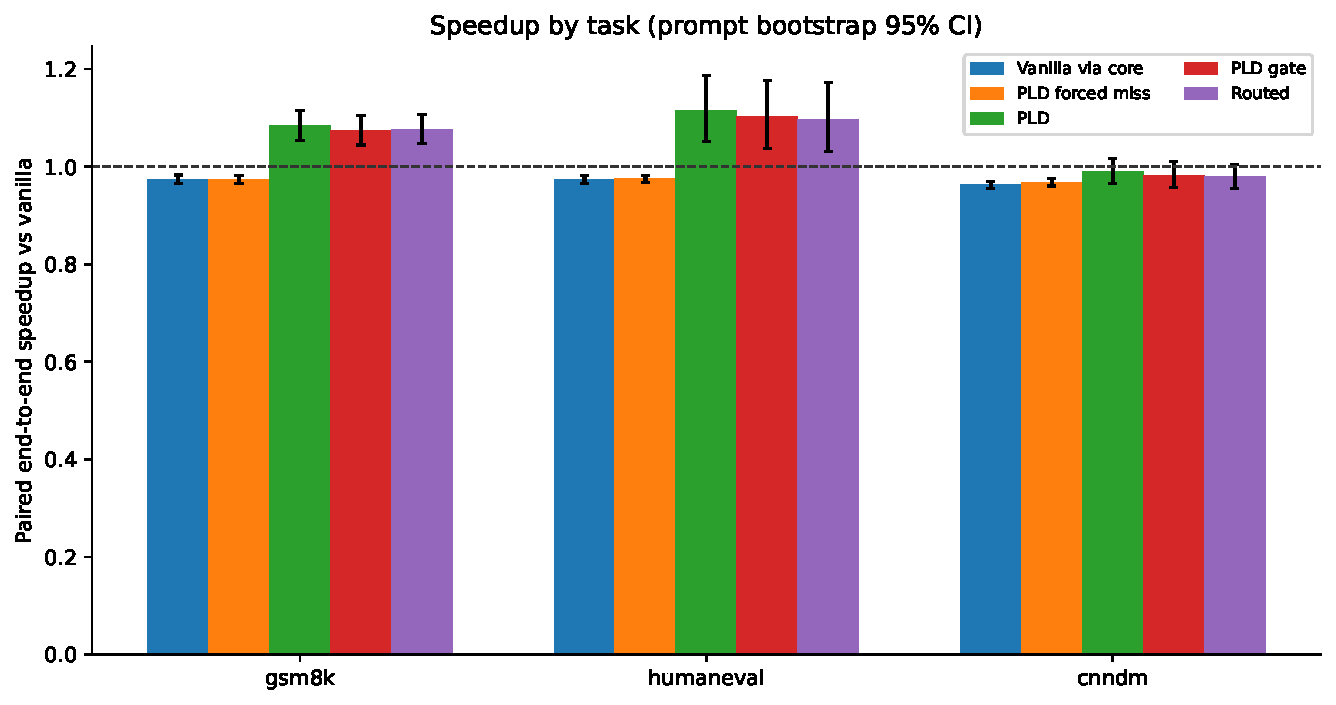
\includegraphics[width=0.88\textwidth]{images/hinh6_speedup_by_task.pdf}
\caption{Speedup end-to-end của các phương pháp theo từng benchmark trong cohort 150 prompt.}
\label{fig:ch5-speedup-task}
\end{figure}

Để làm rõ phân bố ở cấp prompt, Hình~\ref{fig:ch5-paired-distribution} trình bày boxplot speedup paired cho 150 prompt. Trung bình PLD lớn hơn 1 nhưng trung vị chỉ xấp xỉ 1; chỉ 53.3\% prompt nhanh hơn vanilla. Vì vậy, trung bình tổng hợp không có nghĩa PLD cải thiện trên đa số workload với biên độ đồng đều.

\begin{figure}[htbp]
\centering
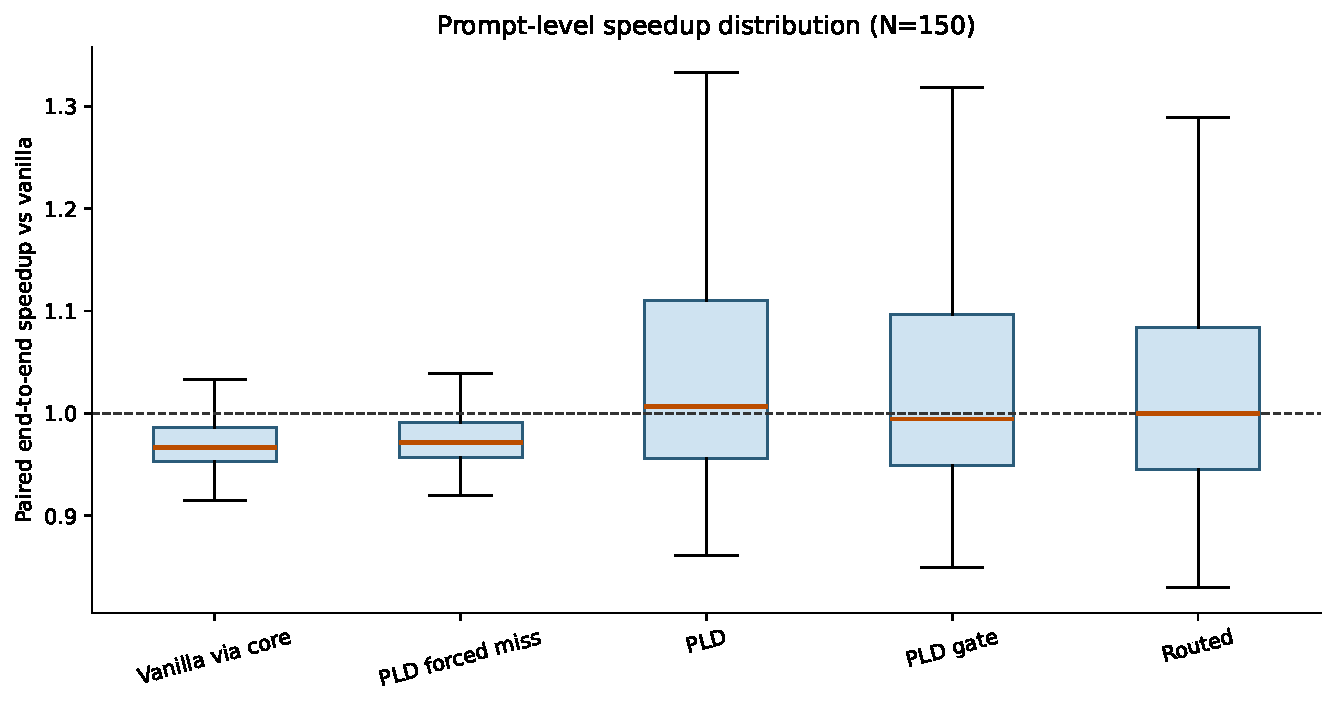
\includegraphics[width=0.88\textwidth]{images/hinh7_paired_speedup.pdf}
\caption{Phân bố speedup end-to-end paired theo prompt; đường đứt đoạn biểu thị hòa vốn \(1.0\times\).}
\label{fig:ch5-paired-distribution}
\end{figure}

Hình~\ref{fig:ch5-speedup-focused} phóng to vùng quanh hòa vốn bằng trục tung thu hẹp từ 0.85 đến 1.20. Các điểm và khoảng tin cậy theo từng tập được vẽ đơn sắc, phân biệt bằng ký hiệu để dễ đọc khi in trắng đen. Khoảng tin cậy là bootstrap theo prompt trong từng tập.

\begin{figure}[htbp]
\centering
\begin{tikzpicture}[x=24cm,y=1.05cm, line cap=round, line join=round, font=\small]
  % Plot range: x=0 maps to 0.85x; x=0.35 maps to 1.20x.
  \draw[->] (0,0.35) -- (0.35,0.35);
  \foreach \x/\lab in {0/0.85,0.05/0.90,0.10/0.95,0.15/1.00,0.20/1.05,0.25/1.10,0.30/1.15,0.35/1.20} {
    \draw (\x,0.35) -- (\x,0.28) node[below=3pt,font=\scriptsize]{\lab};
  }
  \draw[dashed,gray] (0.15,0.48) -- (0.15,3.5);
  \node[anchor=east] at (-0.035,3) {GSM8K};
  \node[anchor=east] at (-0.035,2) {HumanEval};
  \node[anchor=east] at (-0.035,1) {CNN/DailyMail};
  \draw[gray!55] (0,2.5) -- (0.35,2.5);
  \draw[gray!55] (0,1.5) -- (0.35,1.5);
  % PLD: circle; values are mean ratio and prompt-bootstrap 95\% CI.
  \draw (0.205,3.18)--(0.266,3.18); \draw (0.205,3.12)--(0.205,3.24); \draw (0.266,3.12)--(0.266,3.24); \draw[fill=white] (0.234,3.18) circle (1.7pt);
  \draw (0.199,2.18)--(0.340,2.18); \draw (0.199,2.12)--(0.199,2.24); \draw (0.340,2.12)--(0.340,2.24); \draw[fill=white] (0.265,2.18) circle (1.7pt);
  \draw (0.115,1.18)--(0.165,1.18); \draw (0.115,1.12)--(0.115,1.24); \draw (0.165,1.12)--(0.165,1.24); \draw[fill=white] (0.139,1.18) circle (1.7pt);
  % PLD gate: square.
  \draw (0.193,3.00)--(0.255,3.00); \draw (0.193,2.94)--(0.193,3.06); \draw (0.255,2.94)--(0.255,3.06); \draw plot[mark=square*,mark size=1.8pt] coordinates {(0.223,3.00)};
  \draw (0.186,2.00)--(0.329,2.00); \draw (0.186,1.94)--(0.186,2.06); \draw (0.329,1.94)--(0.329,2.06); \draw plot[mark=square*,mark size=1.8pt] coordinates {(0.253,2.00)};
  \draw (0.107,1.00)--(0.159,1.00); \draw (0.107,0.94)--(0.107,1.06); \draw (0.159,0.94)--(0.159,1.06); \draw plot[mark=square*,mark size=1.8pt] coordinates {(0.132,1.00)};
  % Routed: triangle.
  \draw (0.197,2.82)--(0.257,2.82); \draw (0.197,2.76)--(0.197,2.88); \draw (0.257,2.76)--(0.257,2.88); \draw plot[mark=triangle*,mark size=2pt] coordinates {(0.226,2.82)};
  \draw (0.180,1.82)--(0.322,1.82); \draw (0.180,1.76)--(0.180,1.88); \draw (0.322,1.76)--(0.322,1.88); \draw plot[mark=triangle*,mark size=2pt] coordinates {(0.246,1.82)};
  \draw (0.105,0.82)--(0.154,0.82); \draw (0.105,0.76)--(0.105,0.88); \draw (0.154,0.76)--(0.154,0.88); \draw plot[mark=triangle*,mark size=2pt] coordinates {(0.129,0.82)};
  % Monochrome legend.
  \draw (0.015,-0.62)--(0.045,-0.62); \draw[fill=white] (0.030,-0.62) circle (1.7pt); \node[anchor=west] at (0.05,-0.62) {PLD};
  \draw (0.115,-0.62)--(0.145,-0.62); \draw plot[mark=square*,mark size=1.8pt] coordinates {(0.130,-0.62)}; \node[anchor=west] at (0.15,-0.62) {PLD gate};
  \draw (0.245,-0.62)--(0.275,-0.62); \draw plot[mark=triangle*,mark size=2pt] coordinates {(0.260,-0.62)}; \node[anchor=west] at (0.28,-0.62) {Routed};
\end{tikzpicture}
\caption{Speedup theo tập trên vùng tập trung 0.85--1.20\(\times\); trục tung được thu hẹp để thấy rõ chênh lệch quanh đường hòa vốn 1.0\(\times\). Ký hiệu đơn sắc: hình tròn PLD, hình vuông PLD gate, tam giác router; thanh ngang là CI bootstrap 95\%.}
\label{fig:ch5-speedup-focused}
\end{figure}

Các negative control vanilla-via-core và PLD-forced-miss chậm hơn vanilla trực tiếp lần lượt khoảng 3.0\% và 2.8\%. Đây là overhead quan sát được của đường thực thi trong harness, không phải một hiệu chỉnh để cộng vào kết quả PLD. Việc giữ control giúp phân biệt lợi ích do lookup trúng với chi phí nền của speculative path.

\subsection{Layer-skip và router trên cohort riêng}
Trong đánh giá router độc lập gồm 30 prompt ngữ cảnh 384 token, CKA90 với \(K=2\) đạt 0.902\(\times\) vanilla (CI 95\%: 0.875--0.929), trong khi hybrid router đạt 1.045\(\times\) (1.001--1.090) và PLD \(K=2\) được chọn từ development đạt 1.095\(\times\) (1.054--1.139). Trên 14 prompt held-out, CKA90 đạt 0.917\(\times\) (0.880--0.956), router 1.078\(\times\) (1.022--1.142), PLD \(K=2\) 1.134\(\times\) (1.081--1.194). Đây là cohort prepared-input ngắn, một lượt mỗi prompt; nó cho thấy cấu hình layer-skip được khảo sát chậm hơn vanilla, nhưng không thể dùng để kết luận mọi cách chọn lớp hoặc mọi context đều chậm.

\section{Phân tích chi phí và điều kiện hòa vốn}

Speculative decoding chỉ có lợi khi thời gian hoàn thành một cycle đủ thấp so với số token thực sự được phát ra trong cycle đó. Với thời gian vanilla trung bình mỗi token \(T_v\), điều kiện hòa vốn có thể viết \(\mathbb{E}[T_{\mathrm{cycle}}] < \mathbb{E}[N_{\mathrm{emit}}]T_v\). Vì vậy acceptance cao tự nó không chứng minh tăng throughput: một draft tốn thời gian hoặc target verification đắt có thể xóa hết lợi ích của nhiều token được chấp nhận. Mô hình ở Chương~3 được dùng như quan hệ giải thích; phép đo phải tránh cộng chồng các khoảng thời gian đồng thời.

\begin{equation}
T_{\mathrm{cycle}} = T_{\mathrm{draft}} + T_{\mathrm{verify}} + T_{\mathrm{cache}} + T_{\mathrm{lookup}} + T_{\mathrm{control}} + T_{\mathrm{sync}},
\label{eq:ch5-cycle-cost}
\end{equation}

Trong đó các thành phần chỉ được cộng trực tiếp khi được đo trên các khoảng không chồng lấn; các tổng thời gian API host và kernel GPU của profiler không thể cộng cơ học với nhau. Tại benchmark chính, PLD có speedup nhưng router và PLD gate thấp hơn PLD; điều này phù hợp với việc quyết định/fallback bổ sung có chi phí, song benchmark tổng thể không đủ để quy toàn bộ chênh lệch cho riêng một thành phần.

Artifact benchmark lưu số token decode, tổng số verification cycle, số cycle PLD/layer-skip, accepted tokens và tổng decode wall time. Từ các bộ đếm này có thể suy ra một số thống kê gộp như Bảng~\ref{tab:ch5-cycle-stats}. Các giá trị là tỷ số tổng trên 450 lượt prompt/order của mỗi phương pháp, không phải trung bình không trọng số của từng cycle.

Đây là thống kê mô tả gộp được suy ra từ bộ đếm tổng; artifact không lưu thời gian độc lập cho từng cycle. Vì vậy, các giá trị này giúp kiểm tra quan hệ tổng thể giữa số token, số cycle và thời gian, nhưng không xác định chi phí thành phần hay nguyên nhân thời gian của từng cycle.

\begin{table}[htbp]
\centering
\small
\caption{Thống kê cycle gộp suy ra từ raw benchmark paired}
\label{tab:ch5-cycle-stats}
\begin{tabularx}{\textwidth}{@{}>{\centering\arraybackslash}p{2.4cm}>{\centering\arraybackslash}p{2.8cm}>{\centering\arraybackslash}p{3.0cm}>{\centering\arraybackslash}p{2.8cm}>{\centering\arraybackslash}p{2.6cm}@{}}
\toprule
\textbf{Phương pháp} & \textbf{\shortstack{Accepted tokens\\per spec cycle}} & \textbf{\shortstack{Decode tokens\\per verify cycle}} & \textbf{\shortstack{Decode time\\per cycle (ms)}} & \textbf{\shortstack{Vanilla fallback\\cycles}} \\
\midrule
PLD \(K=4\) & 1.134 & 1.217 & 31.82 & 78.5\% \\
Router & 1.125 & 1.227 & 32.51 & 77.5\% \\
\bottomrule
\end{tabularx}
\end{table}

Số candidate draft được đề xuất mỗi cycle không được lưu trong raw file, nên không thể tính trực tiếp đại lượng này hoặc acceptance fraction trên tổng candidates từ artifact hiện tại. Số cycle không draft là phần dư giữa tổng verification cycles và số PLD/layer-skip cycles, dựa trên các trường đếm của harness; vì vậy được xem là thống kê suy ra. Thời gian mỗi cycle được tính bằng tổng decode wall time chia tổng verification cycles. Với vanilla baseline, decode wall time gộp tương ứng khoảng 27.19~ms/token. Thay các thống kê gộp vào \(\mathbb{E}[N_{\mathrm{emit}}]T_v/\mathbb{E}[T_{\mathrm{cycle}}]\) cho decode-only ratio khoảng 1.041 cho PLD và 1.026 cho router; các tỷ số này khớp với pooled decode TPS tính từ cùng token/time totals theo định nghĩa, nên là kiểm tra nhất quán số học chứ không phải dự đoán độc lập. Chúng cũng không thay thế end-to-end paired speedup ở mục~5.4 vì công thức này không tính prefill.

Để khảo sát chi phí ở mức kernel, một phép Nsight riêng chạy trên cùng một prompt 384 token, NF4/FP16, SDPA và giới hạn 32 token. Bảng~\ref{tab:ch5-nsys} tổng hợp thời gian kernel GPU (tổng các kernel có thể chồng lấn) và tổng thời gian API host cho đồng bộ/phát lệnh. Đây là số liệu có instrumentation, không phải end-to-end latency production.

\begin{table}[htbp]
\centering
\small
\caption{Một số số đo Nsight chẩn đoán trên một prompt cố định}
\label{tab:ch5-nsys}
\begin{tabularx}{\textwidth}{@{}Xrrrr@{}}
\toprule
\textbf{Phương pháp} & \textbf{Tổng GPU kernel (ms)} & \textbf{NF4 GEMM (ms)} & \textbf{Dequant (ms)} & \textbf{Sync API (ms)} \\
\midrule
Vanilla & 828.2 & 312.8 & 66.5 & 378.1 \\
PLD \(K=4\) & 811.1 & 400.0 & 54.3 & 270.6 \\
CKA90 \(K=2\) & 951.7 & 451.7 & 40.0 & 376.8 \\
\bottomrule
\end{tabularx}
\end{table}

Số liệu cho thấy thành phần NF4 GEMM, dequant và các lời gọi đồng bộ đều hiện diện đáng kể trong trace. Tuy nhiên, tổng GPU kernel có thể bao gồm overlap, còn synchronize API là thời gian host-side; chúng không phải các thành phần độc lập của critical path. Do đó, từ trace này chỉ có thể mô tả hoạt động quan sát được, chưa thể kết luận dequant hoặc synchronization là nguyên nhân duy nhất gây chậm. Manifest và các tệp xuất Nsight được lưu tại \path{experiments/backend_validation/kernel_profile/}.

\section{Đánh giá bộ nhớ và tính đúng đắn}

\subsection{Bộ nhớ}
Các phương pháp khảo sát không nạp thêm checkpoint draft, nhưng điều đó không đồng nghĩa với không phát sinh thêm VRAM: vẫn có KV cache, activation, vùng làm việc kernel và buffer đã cấp phát. Trong router evaluation 30 prompt (một cohort khác benchmark chính), peak allocated memory trung bình ghi nhận khoảng 2\,107~MiB cho direct vanilla, 2\,110~MiB cho PLD \(K=2\), 2\,111~MiB cho PLD \(K=4\), 2\,112~MiB cho CKA90 \(K=2\), và 2\,113~MiB cho hybrid router. Đây là giá trị trung bình của \texttt{torch.cuda.max\_memory\_allocated}, không phải VRAM NVML/reserved. Chênh lệch nhỏ trong phép đo này không thể khái quát sang mọi context length, backend hoặc cơ chế cấp phát; đây cũng không phải số liệu peak VRAM của cohort 150 prompt.

\subsection{Numerical fidelity và sequence identity}
Benchmark paired chính có exact sequence match 83.3\% cho PLD, PLD gate và router. Phân tích can thiệp trên chính nhóm 25 prompt mismatch (7 GSM8K, 5 HumanEval, 13 CNN/DailyMail) ghi nhận vanilla lặp lại ổn định; trace mặc định có khác biệt digest active KV trước token mismatch, còn verification tuần tự canonical khớp vanilla đủ 48 token trên các prompt này. Kết quả là bằng chứng mạnh cho sự phụ thuộc đường tính toán/cache trong cấu hình NF4 đã thử, nhưng không chứng minh cùng tỷ lệ divergence ở precision hoặc backend khác.

Một kiểm chứng riêng trên 30 prompt, giới hạn 32 token và \(K=4\), phân chia 16 prompt chẩn đoán và 14 held-out cho thấy ảnh hưởng của backend/chế độ thực thi. Mười sáu ID chẩn đoán được lấy từ cohort PLD \(K=4\) ngữ cảnh ngắn đã ghi nhận mismatch trong phép chạy độc lập trước đó; chúng được chọn để khảo sát nguyên nhân sai khác, không lấy ngẫu nhiên từ traffic. Mười bốn ID held-out là các mẫu còn lại trong cùng prepared-input artifact và không được dùng khi chọn nhóm chẩn đoán, nhưng cũng không phải một tập dữ liệu ngoài độc lập. Bảng~\ref{tab:ch5-fidelity} báo cáo sequence match và các chỉ số drift tách biệt.

\begin{table}[htbp]
\centering
\small
\caption{Kết quả numerical fidelity trên cohort 30 prompt; thời gian có tracing chỉ mang tính chẩn đoán}
\label{tab:ch5-fidelity}
\begin{tabularx}{\textwidth}{@{}Xlrrr@{}}
\toprule
\textbf{Cấu hình} & \textbf{Cohort} & \textbf{Exact match} & \textbf{KV/logit drift} & \textbf{Token divergence} \\
\midrule
SDPA, static, batched & Diagnostic (16) & 0/16 & 16/16 & 16/16 \\
SDPA, static, batched & Held-out (14) & 14/14 & 14/14 & 0/14 \\
Eager, static, batched & Diagnostic (16) & 8/16 & 16/16 & 8/16 \\
Eager, static, batched & Held-out (14) & 14/14 & 14/14 & 0/14 \\
SDPA, dynamic, batched & Diagnostic (16) & 0/16 & 16/16 & 16/16 \\
SDPA, dynamic, batched & Held-out (14) & 14/14 & 14/14 & 0/14 \\
SDPA, static, tuần tự & Diagnostic (16) & 16/16 & 0/16 & 0/16 \\
SDPA, static, tuần tự & Held-out (14) & 14/14 & 0/14 & 0/14 \\
\bottomrule
\end{tabularx}
\end{table}

Trong các hàng batched held-out, drift KV/logit được ghi nhận nhưng token sequence vẫn trùng vanilla; đây là ví dụ trực tiếp cho thấy numerical equivalence và sequence identity không tương đương. Mức 0/16 exact match của SDPA batched trên nhóm chẩn đoán là kết quả có điều kiện trên một cohort được chọn vì từng có mismatch, không phải ước lượng tỷ lệ lỗi cho workload tự nhiên. Tương ứng, 14/14 exact match held-out chỉ mô tả 14 mẫu chưa chọn trong cùng artifact; cỡ mẫu nhỏ và nguồn mẫu chung không cho phép kết luận xác suất lỗi thực tế bằng 0. Ở nhóm chẩn đoán, chuyển sang verification tuần tự khôi phục exact match 16/16, đồng thời làm TPS chẩn đoán giảm so với cấu hình batched. Các con số thời gian tại đây có tracing snapshot overhead nên không được so với benchmark production ở mục~5.4.

\subsection{Kiểm tra logic KV cache}
Các test về prefix không bị draft ghi đè, target verification và rollback được mô tả tại Chương~4 và nằm trong \path{tests/test_kv_cache_invariants.py}. Chúng kiểm tra invariant ở mức cấu trúc cache/logical length, trong khi cohort numerical fidelity ở trên đánh giá sai khác tensor và token trên các prompt cụ thể. Hai nhóm bằng chứng bổ sung cho nhau: test invariant không tự bảo đảm logits hoặc chuỗi token luôn tương đương vanilla. Kết quả kiểm thử chỉ nên gắn với log chạy tương ứng; không suy rộng sang các cấu hình chưa chạy.

\section{Thảo luận và giới hạn}

Bảng~\ref{tab:ch5-rq} tóm tắt câu trả lời thực nghiệm trong phạm vi các cohort hiện có.

\begin{table}[htbp]
\centering
\small
\caption{Tổng hợp kết quả theo câu hỏi nghiên cứu}
\label{tab:ch5-rq}
\begin{tabularx}{\textwidth}{@{}p{1.3cm}X@{}}
\toprule
\textbf{Câu hỏi} & \textbf{Kết luận có giới hạn theo bằng chứng} \\
\midrule
RQ1 & PLD tăng tốc trung bình trên cohort 150 prompt (1.063\(\times\)), nhưng hiệu quả phụ thuộc tập dữ liệu; CNN/DailyMail đạt 0.989\(\times\). CKA90/K2 chậm hơn vanilla trong cohort router 30 prompt đã thử. \\
RQ2 & Draft, verify, lookup, điều khiển và đồng bộ cùng ảnh hưởng thời gian cycle. Nsight cho thấy các hoạt động GEMM, dequant và sync, nhưng phép profiling đơn lẻ chưa xác định critical path nhân quả. Acceptance cao không bảo đảm tăng tốc. \\
RQ3 & Với NF4, batched execution có các trường hợp KV/logit drift và token divergence; verification tuần tự khớp vanilla trên cohort fidelity đã thử nhưng chậm hơn trong phép đo có tracing. Kết luận không thay thế kiểm chứng trên precision/backend khác. \\
RQ4 & Router tăng tốc so với vanilla trong benchmark chính (1.050\(\times\)) nhưng thấp hơn PLD (tỷ số paired 0.989; CI 0.985--0.993). Router hiện chưa chứng minh lợi ích so với fixed PLD trong giao thức này. \\
\bottomrule
\end{tabularx}
\end{table}
Các giới hạn chính gồm: benchmark hiệu năng chính chạy trên một GPU và một cấu hình NF4/SDPA; tốc độ biến thiên theo prompt và tập dữ liệu; exact sequence match thấp hơn 100\% trong phương pháp suy đoán; các phép router, fidelity và profiling dùng cohort/cấu hình riêng; profiling có instrumentation; và chưa có cơ sở để khái quát sang mô hình, GPU, precision hay backend khác. Các thí nghiệm context/backend exploratory cũng không được trộn vào kết quả xác nhận của benchmark 150 prompt.

Trong điều kiện GPU VRAM hạn chế, một kỹ thuật speculative decoding đáng sử dụng khi đồng thời thỏa ba điều kiện có thể kiểm chứng: (1) tổng chi phí cycle đủ thấp so với số token được phát ra, thay vì chỉ có acceptance cao; (2) nó cải thiện trên baseline cố định mạnh nhất đã đo, không chỉ vượt vanilla; và (3) mức speedup đáp ứng yêu cầu numerical fidelity/sequence identity của ứng dụng. Trong thí nghiệm này, PLD vượt vanilla trung bình nhưng có mismatch token và không nhanh hơn trên CNN/DailyMail; router vẫn dưới PLD; verification tuần tự khôi phục sequence identity trong cohort fidelity nhưng tốn thời gian hơn. Vì vậy, lựa chọn thực tế phụ thuộc vào workload, ngân sách latency và yêu cầu chính xác đầu ra.

\clearpage
\chapter{Giải mã suy đoán exact trên mô hình NF4 không dùng thêm bộ nhớ GPU}\label{chap:b2}

% Macro cục bộ cho chương này (không đụng tới packages.tex).
\providecommand{\code}[1]{\texttt{\detokenize{#1}}}
\providecommand{\ci}[3]{#1 [#2,\,#3]}

Chương này trình bày phần nghiên cứu mở rộng sau các phép đo ở Chương 5: thay vì chấp nhận rằng speedup của PLD đi kèm đầu ra có thể lệch khỏi vanilla, chương xây dựng một vòng giải mã suy đoán \emph{exact} cho mô hình lượng tử hóa NF4 và đánh giá nó với giao thức tách riêng tập phát triển và hai cohort held-out dùng đúng một lần. Toàn bộ kết quả là bằng chứng thực nghiệm hữu hạn trên một GPU, chưa phải chứng minh.

\section{Động lực và mục tiêu}
Giải mã suy đoán tăng tốc suy luận bằng cách đề xuất vài token tương lai rồi kiểm tra chúng song song trong một lần chạy mô hình \cite{leviathan2023fast,chen2023accelerating}. Với greedy, đầu ra \emph{về nguyên tắc} bằng đầu ra giải mã tuần tự. Trên thực tế, ``bằng nhau'' chỉ đúng nếu lần chạy theo khối cho logits và KV giống hệt bước một-token. Các toán tử trong mô hình chọn kernel theo hình dạng đầu vào, nên đầu ra theo khối có thể chỉ gần đúng và quỹ đạo có thể rẽ nhánh; Mục~\ref{sec:attrib} cho thấy toán tử nào thực sự gây lệch trong ngăn xếp bitsandbytes 0.50.0 và PyTorch SDPA. Trong giao thức trước của kho mã này, Prompt Lookup Decoding (PLD) \cite{saxena2024promptlookup} trên NF4 \cite{dettmers2023qlora} chỉ khớp đầu ra không suy đoán ở $83.3\%$ chuỗi ($N{=}150$) và $21/60$ ở một phép so sánh backend sau đó.

\paragraph{Mục tiêu.} Cho một tham chiếu chính xác (greedy bitsandbytes M=1 không sửa đổi), xây dựng vòng giải mã suy đoán (i) cho đúng chuỗi token tham chiếu, (ii) không dùng mô hình draft và không dùng thêm bộ nhớ GPU đáng kể, (iii) nhanh hơn tham chiếu. Chúng tôi đặt tính đúng đắn lên trước tốc độ: tốc độ chỉ có nghĩa khi (i) đã giữ.

\paragraph{Đóng góp.}
\begin{enumerate}[nosep]
\item Một vòng giải mã exact B2 và các thành phần của nó (Mục~\ref{sec:method}), kèm cách đọc tính đúng đắn theo toán tử và phân loại rõ phần nào theo cấu trúc mã, phần nào chỉ có bằng chứng thực nghiệm (Mục~\ref{sec:argument}).
\item Hai phát hiện: (i) trong ngăn xếp bitsandbytes 0.50.0 và PyTorch, kiểm tra theo khối làm lệch quỹ đạo chủ yếu qua attention và LM head chứ không qua phép chiếu NF4 (Mục~\ref{sec:attrib}); (ii) mã nguồn CUDA của bitsandbytes đọc theo nghĩa đen cộng tích lũy tuần tự, nhưng bản nhị phân thật khớp thứ tự cộng theo cặp của kernel Triton (Mục~\ref{sec:order}).
\item Bằng chứng nhiều tầng: token và KV bitwise từng bước, quay lui, EOS, ngữ cảnh tới $3071$ token, ba kích cỡ mô hình, hai cohort held-out đăng ký trước (Mục~\ref{sec:results}).
\item Các kết quả bất lợi và âm có ghi chép: baseline biên dịch nhanh hơn, hướng cải thiện không hiệu quả (Mục~\ref{sec:negative}).
\end{enumerate}
Công trình gần nhất chúng tôi biết là LLM-42 \cite{gond2026llm42}, dùng vòng decode--verify--rollback để đảm bảo xác định ở mức hệ thống phục vụ trên FP16 nhiều GPU; chúng tôi giải một bài toán khác ở mức số học trong lượng tử hóa 4-bit trên một GPU tiêu dùng.

\section{Bài toán và định nghĩa}
Cố định trọng số, trạng thái lượng tử hóa, phiên bản thư viện, kiến trúc GPU, cài đặt attention, thủ tục prefill, kiểu và dung lượng cache, quy tắc chọn token khi bằng nhau và quy tắc EOS. Gọi $R(S_t,x_t)=(z_t,S_{t+1})$ là bước chuyển một-token tham chiếu: chạy \code{model(x)} với bitsandbytes không sửa đổi, $x$ có hình dạng $(1,1)$. Trạng thái $S_t$ gồm mọi thứ ảnh hưởng tới lần chạy sau (mọi mục KV, độ dài logic, vị trí). \emph{Exact} nghĩa là chuỗi token sinh ra bằng chuỗi do $R$ sinh, và (ở các kiểm tra mạnh hơn) KV cũng bằng từng bit tại mọi bước.

Chúng tôi phân biệt hai tham chiếu. \textbf{B1} là greedy với lịch hình dạng cố định (mọi phép toán được đệm về cùng số hàng vật lý); nó làm đổi số học của mô hình nên không bằng greedy gốc. \textbf{B2} là greedy bitsandbytes gốc; chỉ B2 là mục tiêu của chương này.

\section{Phương pháp}\label{sec:method}
Mỗi chu kỳ gồm: tra n-gram để đề xuất tối đa $k{=}2$ token; chạy mô hình trên $1{+}\#\text{đề xuất}$ hàng; chấp nhận tiền tố khớp dài nhất; quay lui KV phần bị loại. Các thành phần:

\paragraph{Kernel NF4 $M{=}3$ (tùy chọn, chỉ để tăng tốc).} \code{_fused_nf4_m3_kernel} (Triton \cite{tillet2019triton}) xử lý ba hàng activation với ba bộ cộng dồn độc lập, cùng một trọng số giải lượng tử dùng chung. Mỗi lane cộng $32$ tích fp16 (\code{mul.rn.f16x2}), tích lũy trong fp32 theo từng cặp, rồi gộp $32$ lane bằng cây dịch $16,8,4,2,1$. Chạy với \code{enable_fp_fusion=False}. Mã không có câu lệnh nào đọc dữ liệu của hàng khác nên đầu ra từng hàng chỉ phụ thuộc hàng đó. Kernel này \emph{không cần cho tính exact}: trong bitsandbytes 0.50.0 các phép chiếu NF4 chuẩn đã cho đầu ra từng hàng bằng bước $M{=}1$ (Mục~\ref{sec:attrib}), và B2 lười không dùng kernel Triton vẫn khớp BNB ở $10/10$ prompt dev (token và KV). Kernel chỉ giúp tăng tốc: $1.161\times$ so với $1.117\times$ khi dùng phép chiếu chuẩn (10 prompt GSM8K dev).

\paragraph{Phép toán từng hàng.} RMSNorm, LM head và attention được gọi riêng cho từng hàng: attention gọi \code{scaled_dot_product_attention} một lần cho mỗi hàng với K/V cắt đúng $L_t{+}i{+}1$ vị trí, không mặt nạ, \code{enable_gqa=True}, nên hình dạng giống lời gọi một-token.

\paragraph{Quay lui và quay về $M{=}1$.} Cache tĩnh chỉ trả về $[0,\text{seq\_len})$ nên cắt độ dài logic là đủ để các mục dư không bao giờ được đọc trước khi bị ghi đè. Khi không có đề xuất, vòng chạy đúng bước $M{=}1$ gốc (không lịch, không kernel Triton) bằng cách hoán đổi \code{forward} từng module giữa bản gốc và bản đã vá; lịch được vào một lần cho cả lượt sinh.

\paragraph{LM head lười.} Chiếu LM head cho từng hàng chỉ cho tới hàng bị loại đầu tiên: các hàng sau không bao giờ được dùng và không ghi trạng thái, nên bỏ qua chúng không đổi kết quả.

\begin{algorithm}[t]
\caption{Một lượt sinh của B2 (rút gọn)}\label{alg:b2}
\begin{algorithmic}[1]
\Require prompt, ngân sách $N$, $k{=}2$
\State prefill bằng BNB gốc; $\mathit{pending}\gets$ token đầu của greedy
\While{chưa đủ $N$ token và \textbf{chưa} gặp EOS}
  \State $C\gets$ PLD(lịch sử $+\ \mathit{pending}$, $\le k$ token)
  \If{$C=\emptyset$}\Comment{quay về bước gốc}
    \State chạy BNB $M{=}1$ trên $\mathit{pending}$; $\mathit{pending}\gets$ argmax
  \Else
    \State hoán đổi sang bản vá; chạy decoder trên $[\mathit{pending}]\,{+}\,C$ (một lần)
    \For{$i=0,1,\dots$} \Comment{LM head lười}
      \State $p_i\gets \operatorname{argmax}\,\mathrm{lm\_head}(h_i)$; \textbf{nếu} $i<|C|$ \textbf{và} $p_i\neq C_i$ \textbf{thì} dừng
    \EndFor
    \State phát $\mathit{pending}$ và các $C_j$ được chấp nhận; cắt KV về độ dài đã commit
    \State $\mathit{pending}\gets p_{\text{hàng cuối đã tính}}$
  \EndIf
\EndWhile
\end{algorithmic}
\end{algorithm}

\section{Lập luận về tính đúng đắn}\label{sec:argument}
Gọi \emph{tính bằng nhau theo hàng} (RE) là: với khối bắt đầu từ trạng thái bằng tham chiếu, hàng $i$ của mọi tensor trung gian bằng từng bit với tensor tương ứng của $R$ áp dụng lần lượt $x_0,\dots,x_i$, và KV ghi tại vị trí $L_t{+}i$ cũng bằng. Từ RE, quy nạp theo chu kỳ cho kết quả: (1) logits hàng $i$ bằng tham chiếu; (2) tiền tố được chấp nhận và $\mathit{pending}$ bằng chuỗi greedy; (3) cắt độ dài logic giữ lại đúng $[0,L_t{+}j{+}1)$; (4) chu kỳ không đề xuất chính là $R$. Giả thiết duy nhất không thuộc cấu trúc là RE ở từng toán tử.

\begin{table}[t]
\centering\small
\caption{Trạng thái lập luận theo toán tử. \textbf{[S]}: theo cấu trúc mã; \textbf{[E]}: chỉ có bằng chứng thực nghiệm; \textbf{[O]}: còn mở.}\label{tab:ops}
\begin{tabularx}{\textwidth}{@{}>{\raggedright\arraybackslash}p{0.25\textwidth}>{\raggedright\arraybackslash}X>{\raggedright\arraybackslash}p{0.3\textwidth}@{}}
\toprule
Toán tử & Cơ sở & Nhãn\\\midrule
Embedding, ghi KV, argmax, LM head & gọi từng hàng hoặc sao chép byte & [S]\\
RMSNorm & gọi riêng từng hàng, giống tham chiếu & [S]\\
Attention & một lời gọi SDPA mỗi hàng, cùng hình dạng, bố cục & [S] nếu dispatch chỉ phụ thuộc hình dạng/stride; [O]\\
Rotary, residual, SiLU$\cdot$mul & phép toán theo phần tử; chưa kiểm riêng bản vector hóa & [S]/[O]\\
Phép chiếu NF4 (252) & bitsandbytes chuẩn: $0$ lệch trong $9.9\times10^{8}$ phần tử khi gọi ba hàng so với từng hàng; kernel Triton tùy chọn có ba bộ cộng dồn độc lập & [E]; [S]+[E] cho kernel Triton\\
\bottomrule
\end{tabularx}
\end{table}

\subsection{Thứ tự rút gọn của kernel bitsandbytes}\label{sec:order}
Phần này chỉ liên quan tới kernel Triton tùy chọn: nó cho biết khi nào kernel đó thay được kernel bitsandbytes mà không đổi kết quả.
Mã nguồn bitsandbytes 0.50.0 (\texttt{kgemm\_\allowbreak 4bit\_\allowbreak inference\_\allowbreak naive}) cộng tuần tự từng tích fp16 trong mỗi lane, còn kernel Triton của chúng tôi cộng từng cặp tích liền kề trước. Theo số học IEEE hai thứ tự này khác nhau. Chúng tôi mô phỏng cả hai thứ tự trong fp32 trên $28\,672\,000$ đầu ra ngẫu nhiên đuôi nặng (năm lớp, đủ bảy phép chiếu). Kernel bitsandbytes thật và kernel Triton \emph{đều khớp mô phỏng theo cặp ở $28\,672\,000/28\,672\,000$ đầu ra} và đều khác mô phỏng tuần tự ở $398$ đầu ra; phép thử đủ nhạy để phân biệt hai thứ tự. Cận trên $95\%$ của tỷ lệ lệch mỗi đầu ra khoảng $1.0\times10^{-7}$ (quy tắc ba). Chúng tôi chưa giải thích được vì sao bản nhị phân khác mã nguồn đã đọc, nên mọi lần nâng cấp bitsandbytes phải chạy lại phép mô phỏng này.

\section{Thiết lập thực nghiệm}
\paragraph{Môi trường.} Qwen2.5-3B-Instruct \cite{qwen2024qwen25}, revision \code{aa8e7253...}, bitsandbytes 0.50.0 (NF4, lượng tử hóa kép, tính toán fp16), Triton 3.6.0, PyTorch 2.11.0, transformers 5.14.1, một GPU RTX 4050 Laptop 6~GB, batch 1, greedy, $k{=}2$, PLD với n-gram $\le 3$, $128$ token sinh nếu không ghi khác.

\paragraph{Dữ liệu và giao thức.} Tập \emph{dev} (GSM8K, HumanEval, CNN/DM) dùng để phát triển và chọn cấu hình. Hai cohort \emph{held-out} GSM8K, chỉ số test $300$--$349$ và $400$--$449$, được đóng băng theo chỉ số công khai, kiểm tra không trùng ID/prompt với mọi benchmark cục bộ, đăng ký cấu hình trước khi chạy và chỉ dùng \emph{một lần}; chúng không được dùng để chọn cấu hình. Việc này không loại trừ dữ liệu công khai đã lọt vào dữ liệu huấn luyện mô hình.

\paragraph{Chỉ tiêu.} (i) Token khớp tham chiếu BNB eager; (ii) băm SHA256 của KV tại mọi tiền tố không-terminal; (iii) tốc độ $=$ thời gian BNB eager $/$ thời gian phương pháp, trung vị trên $2$--$3$ vòng xoay thứ tự, trung bình nhân giữa các prompt kèm khoảng tin cậy $95\%$ bootstrap theo prompt ($10^4$ lần, seed 0). Thời gian gồm cả prefill.

\section{Kết quả}\label{sec:results}
\subsection{Tính đúng đắn}
\begin{table}[t]
\centering\small
\caption{Bằng chứng tính đúng đắn của B2 (so với greedy bitsandbytes gốc).}\label{tab:exact}
\begin{tabularx}{\textwidth}{@{}Xrl@{}}
\toprule
Kiểm tra & Quy mô & Kết quả\\\midrule
Held-out GSM8K $300$--$349$ (token) & 50 prompt & $50/50$\\
Held-out GSM8K $400$--$449$ (token và KV từng bước) & 50 prompt & $50/50$ và $50/50$\\
Dev GSM8K, HumanEval (token) & 60 prompt & $60/60$\\
Ngữ cảnh $512$--$3071$ token (token và KV) & 12 prompt & $12/12$\\
Kết thúc bằng EOS, sinh tới $384$ token (token và KV) & 18 prompt & $18/18$\\
Quay lui/loại tại các vị trí $0,1$, nhiều chu kỳ (3 prompt trên 3B, 1 prompt mỗi mô hình 0.5B và 1.5B) & 5 kịch bản & đạt\\
Qwen2.5-0.5B và 1.5B (token và KV) & 10 prompt mỗi mô hình & $10/10$\\
Phép chiếu NF4 trên activation thật & 252 module, $9.29$M phần tử & bằng từng bit\\
\bottomrule
\end{tabularx}
\end{table}

\subsection{Toán tử nào làm vỡ tính exact}\label{sec:attrib}
Để biết sai lệch của kiểm tra theo khối đến từ đâu, chúng tôi chạy đường \emph{chuẩn} (không vá) của HF với bitsandbytes 0.50.0 trên các khối ba token teacher-forced, đặt ở trạng thái tuần tự chính xác (20 prompt GSM8K dev, 16 khối mỗi prompt, $960$ hàng). Với mỗi toán tử ta ghi đầu vào thật của nó khi chạy khối, rồi gọi lại \emph{cùng toán tử trên cùng đầu vào} từng hàng một và so sánh từng bit (Bảng~\ref{tab:attrib}). Chỉ attention và LM head lệch đáng kể; các phép chiếu NF4 chuẩn khớp từng hàng ở mọi phần tử đã kiểm, và RMSNorm gần như khớp. Hệ quả cuối-cuối: $960/960$ hàng logits không bằng từng bit, $4/960$ hàng ($0.42\%$) đổi argmax (độ chênh top-1/top-2 của chúng $\le 0.125$, một hàng là hòa tuyệt đối); trung vị của độ lệch logits lớn nhất là $0.22$ và giá trị lớn nhất là $1.36$. Vì vậy trong ngăn xếp này tính exact bị phá bởi attention và LM head chứ không phải phép chiếu 4-bit, và B2 xử lý chính các toán tử đó bằng lời gọi từng hàng. Kết quả chỉ cho một phiên bản bitsandbytes, một GPU và $M{=}3$: bitsandbytes 0.50.0 chọn kernel NF4 cho $M$ nhỏ theo ngưỡng riêng, và phiên bản khác có thể khác.

\begin{table}[t]
\centering\small
\caption{So sánh từng bit giữa toán tử gọi ba hàng và gọi từng hàng trên cùng đầu vào (đường chuẩn, 960 hàng).}\label{tab:attrib}
\begin{tabular}{@{}lrrr@{}}
\toprule
Toán tử & Số phần tử & Lệch từng bit & Tỷ lệ\\\midrule
Phép chiếu NF4 (7 loại) & $990\,904\,320$ & $0$ & $0$\\
RMSNorm trong lớp & $141\,557\,760$ & $87$ & $6.1\times10^{-7}$\\
RMSNorm cuối & $1\,966\,080$ & $0$ & $0$\\
LM head & $145\,858\,560$ & $281\,534$ & $1.9\times10^{-3}$\\
Attention (SDPA) & $70\,778\,880$ & $13\,196\,548$ & $0.186$\\
\bottomrule
\end{tabular}
\end{table}

\subsection{Tốc độ và so sánh với B1}
Trên held-out $300$--$349$ (phiên bản B2 với LM head đầy đủ), B2 đạt \ci{1.117}{1.100}{1.135}$\times$ so với BNB eager, khớp $50/50$ prompt; B1 (kernel Triton ba hàng, lịch hình dạng cố định) đạt \ci{1.108}{1.087}{1.130}$\times$ nhưng chỉ khớp BNB gốc ở $24/50$ prompt. Tỷ số B2/B1 là \ci{1.008}{0.995}{1.022}: hai bên không phân biệt được về tốc độ, khác biệt nằm ở tính exact. Trên held-out $400$--$449$ với B2 lười (Hình~\ref{fig:methods}): B2 lười đạt \ci{1.154}{1.136}{1.172}$\times$ so với \ci{1.097}{1.080}{1.113}$\times$ của B2 LM head đầy đủ (lười/đầy đủ $=\ci{1.052}{1.044}{1.060}$), không prompt nào dưới BNB. Trên dev, B2 lười đạt \ci{1.166}{1.145}{1.188}$\times$ (GSM8K) và \ci{1.249}{1.208}{1.296}$\times$ (HumanEval), mỗi cohort $30$ prompt.

\begin{figure}[t]
\centering
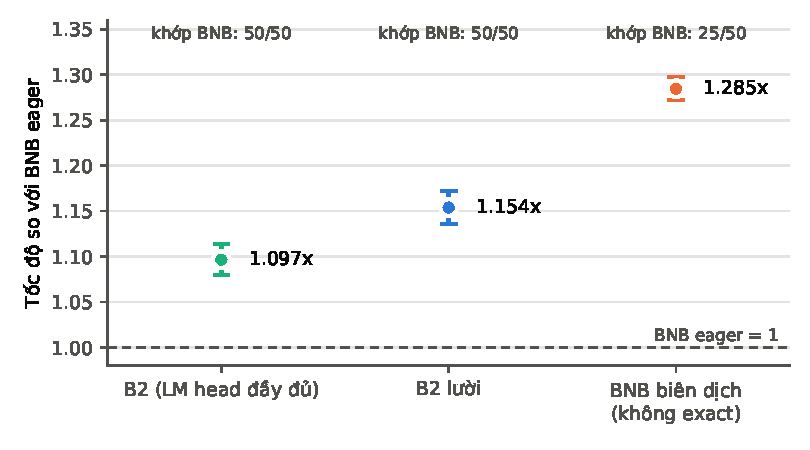
\includegraphics[width=0.78\textwidth]{images/tr_methods_heldout2.pdf}
\caption{Tốc độ so với BNB eager trên held-out GSM8K $400$--$449$ (50 prompt; điểm là trung bình nhân, thanh là khoảng tin cậy $95\%$). Dòng trên cùng ghi số prompt có token khớp BNB eager. BNB biên dịch nhanh hơn nhưng chỉ khớp $25/50$.}\label{fig:methods}
\end{figure}

\subsection{So sánh với baseline biên dịch}\label{sec:compiled}
Một vòng decode BNB với \code{StaticCache} và \code{torch.compile} (mode \code{reduce-overhead}) nhanh hơn BNB eager \ci{1.285}{1.272}{1.297}$\times$ trên held-out $400$--$449$, đo cạnh nhau cùng lượt chạy. Tuy nhiên token của nó chỉ khớp eager ở $25/50$ prompt, tức không phải tham chiếu bitwise. B2 lười đạt $0.907\times$ [$0.893$, $0.920$] tốc độ của nó và chậm hơn ở $49/50$ prompt (trên dev: $0.82\times$, $12$ prompt). Vì vậy luận điểm đúng của B2 là ``exact so với BNB eager, nhanh hơn eager khoảng $1.1$--$1.25\times$'', không phải ``nhanh hơn baseline mạnh''. Chưa thử kết hợp compile với giải mã suy đoán; nó sẽ đổi số học và đòi hỏi định nghĩa lại tham chiếu.

\subsection{Ngữ cảnh dài và các mô hình khác}
\begin{figure}[t]
\centering
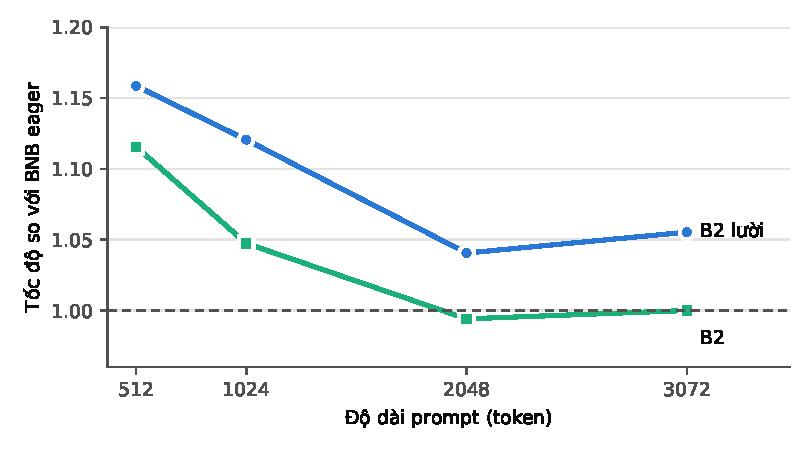
\includegraphics[width=0.78\textwidth]{images/tr_context_length.pdf}
\caption{Tốc độ so với BNB eager theo độ dài prompt (3 prompt dev mỗi độ dài, tóm tắt nhiều bài CNN/DM ghép lại).}\label{fig:context}
\end{figure}
Token và KV khớp ở mọi độ dài tới $3071$ token, nhưng tốc độ giảm (Hình~\ref{fig:context}): B2 lười còn $1.04$--$1.06\times$ ở $2048$--$3072$ token. Chi phí một forward gần như không đổi theo độ dài (wall: BNB $M{=}1$ $23.2\to23.5$ ms), nên nguyên nhân đã đo là acceptance thấp trên tác vụ tóm tắt ($0.24$--$0.29$ ở $3072$ so với $0.32$--$0.64$ ở $512$) và prefill chung ($1.1$ s ở $3072$ token) làm loãng tỷ lệ; chưa có prompt dài mà acceptance cao để tách hoàn toàn hai yếu tố. Trên Qwen2.5-0.5B và 1.5B (10 prompt dev) B2 lười đạt $1.243\times$ và $1.163\times$, token và KV khớp $10/10$.

\subsection{Bộ nhớ}
Ở cùng dung lượng cache tĩnh, đỉnh bộ nhớ cấp phát của B2 chỉ lớn hơn BNB eager $0.07$~MiB ($2007.90$ so với $2007.97$ MiB ở prompt $75$ token; $2994.61$ so với $2994.68$ MiB ở $3071$ token); đỉnh dự trữ và bộ nhớ thiết bị dùng giống hệt nhau, và không có mô hình draft. Mỗi phương pháp chạy trong một tiến trình riêng, đo ở lượt thứ hai.

\subsection{Phân tích chi phí}
Một forward khối $M{=}3$ tốn $37.1$ ms, gấp $1.65$ lần một bước $M{=}1$ ($22.5$ ms), nên block chỉ có lợi khi sinh trên $1.65$ token mỗi chu kỳ (acceptance khoảng $33\%$ với hai đề xuất); trung bình $1.86$ token mỗi chu kỳ khối và $73\%$ chu kỳ phải quay về bước gốc, khớp với mức tăng tốc khoảng $12$--$15\%$. LM head bf16 tốn khoảng $3.3$ ms mỗi hàng và là phần lớn của chênh lệch GPU, nên chiếu lười có ích. Cả hai loại forward bị giới hạn bởi CPU khởi chạy kernel ($84\%$ thời gian một bước $M{=}1$ là enqueue CPU), điều này cũng giải thích vì sao baseline biên dịch (giảm overhead CPU) nhanh hơn.

\subsection{Thăm dò: chụp CUDA graph (ước lượng, chưa cài đặt)}
Chúng tôi chụp thô một bước decode $M{=}1$ của mô hình bitsandbytes eager với \code{StaticCache} bằng CUDA graph (không \code{torch.compile}, cùng các kernel): chụp được, logits bằng từng bit ở $64/64$ bước, và chi phí giảm từ $22.5$ xuống $17.3$ ms mỗi bước ($1.30\times$). Khối chuẩn ba hàng (không exact) tốn $27.4$ ms ở chế độ eager và $23.9$ ms trong graph. Ghép với mô phỏng đã hiệu chỉnh, một vòng B2 chạy phần thân decoder trong graph (các phép từng hàng nằm trong graph nên không còn tốn CPU) với LM head lười chạy ngoài graph cho tốc độ ước lượng $1.36$--$1.48\times$ so với eager, nhưng chỉ $1.04$--$1.14\times$ so với một baseline graph exact. Đây là dự đoán từ mô hình chi phí (chi phí decoder ba hàng trong graph $21.7$--$24.0$ ms ước từ số đo kernel), chưa được cài đặt, nên không phải kết quả đã đo của B2.

\section{Các kết quả bất lợi và hướng không hiệu quả}\label{sec:negative}
\begin{itemize}[nosep]
\item \textbf{Chọn n-gram.} Quét độ dài n-gram $2$--$5$ chênh dưới $2\%$ và nằm trong nhiễu đo. Bảy chính sách chọn draft (lọc đề xuất yếu, bỏ phiếu giữa các lần khớp, ngưỡng lặp) đều khớp BNB; lọc đề xuất yếu không nhanh hơn dù giảm gần một nửa số khối, và bỏ phiếu so với chính sách gốc cho tỷ số \ci{1.002}{0.998}{1.007} trên $80$ prompt dev chưa dùng để chọn. Giữ chính sách gốc.
\item \textbf{Giảm chi phí CPU.} Gọi thẳng kernel Triton đã biên dịch cho kết quả bằng nhau từng bit nhưng không nhanh hơn ($7.22$ so với $7.59$ ms cho $252$ phép chiếu); các điểm nóng còn lại là chuỗi phép PyTorch nhỏ ở RMSNorm và attention từng hàng, không thể giảm mà không đổi tập kernel.
\item \textbf{Khối lớn hơn.} Mô phỏng (chạy PLD trên chuỗi tham chiếu đã ghi, chi phí mỗi hàng hiệu chỉnh khớp $K{=}2$ đo được) dự đoán $K{=}3,4$ thay đổi từ $-1\%$ đến $+2.6\%$ so với $K{=}2$ (tới $+4.1\%$ nếu chi phí mỗi hàng giảm một nửa); không đáng viết kernel mới. Đây là dự đoán từ mô hình tuyến tính, chưa kiểm bằng thực nghiệm.
\item \textbf{Quay về bước gốc.} Quay về $M{=}1$ khi không có đề xuất đưa tốc độ từ $0.91$--$0.97\times$ lên $1.06$--$1.15\times$ trên các cohort dev nhỏ; đây là thay đổi đóng góp lớn nhất.
\end{itemize}

\section{Giới hạn và mối đe dọa tính hợp lệ}
\begin{itemize}[nosep]
\item \textbf{Phạm vi.} Một GPU và bộ công cụ, chủ yếu một họ mô hình (Qwen2), một backend lượng tử hóa (bitsandbytes), batch 1, greedy, $k{=}2$. Kết quả không áp dụng được cho lấy mẫu, batch lớn hay các lược đồ lượng tử hóa khác.
\item \textbf{Chứng minh.} Tính exact dựa trên bằng chứng hữu hạn. Còn mở: bằng kernel bitsandbytes trên mọi đầu vào, độc lập của dispatch PyTorch với số hàng, độ ổn định qua phiên bản Triton/ptxas/CUDA và GPU, kiểm ở mức PTX.
\item \textbf{Chọn cấu hình.} Cấu hình được chọn trên dev; hai cohort held-out không dùng để chọn, nhưng cohort $400$--$449$ được dùng để đánh giá riêng biến thể B2 lười đã cố định trước đó, và cohort $300$--$349$ chỉ đánh giá biến thể LM head đầy đủ.
\item \textbf{Khoảng tin cậy.} Chỉ phản ánh biến thiên giữa các prompt đã chọn, không phải toàn bộ workload. Tốc độ tuyệt đối phụ thuộc cohort ($1.23\times$ ở HumanEval $0$--$19$ nhưng $1.31\times$ ở $20$--$49$).
\item \textbf{Baseline.} Tốc độ chỉ so với BNB eager; baseline biên dịch nhanh hơn nhưng không exact.
\end{itemize}

\section{Tóm tắt chương}
Với Qwen2.5-3B NF4 trên một GPU tiêu dùng, B2 tái tạo đúng từng token và KV của greedy bitsandbytes, không dùng thêm bộ nhớ đáng kể và nhanh hơn eager khoảng $12$--$15\%$ trên hai cohort held-out; mức tăng khiêm tốn và bị giới hạn bởi chi phí khởi chạy CPU và acceptance của PLD. Giá trị chính nằm ở tính exact và quy trình bằng chứng chứ không ở tốc độ. Hướng tiếp theo gồm kiểm ở mức PTX và trên GPU/phiên bản Triton khác, mở rộng sang backend lượng tử hóa và họ mô hình khác, và chứng minh hợp đồng toán tử.

Mã, bằng chứng thô và kịch bản tái lập nằm trong kho mã (thư mục \texttt{experiments}).

\clearpage
\chapter{Kernel 4-bit bất biến theo số hàng cho giải mã suy đoán exact}\label{chap:kernel}

\providecommand{\code}[1]{\texttt{\detokenize{#1}}}
\providecommand{\ci}[3]{#1 [#2,\,#3]}

Chương~\ref{chap:b2} xây dựng vòng giải mã exact B2 bằng cách gọi từng hàng các toán tử nhạy với hình dạng. Cách đó giữ đúng chuỗi của bitsandbytes gốc nhưng bỏ phần lớn lợi ích của việc kiểm tra theo khối: trọng số được đọc lại cho mỗi hàng. Chương này đi theo hướng ngược lại, trả lời RQ6: \emph{có thể thiết kế các kernel 4-bit mà kết quả của từng hàng không phụ thuộc vào số hàng $M$ trong khối, sao cho kiểm tra theo khối vừa exact vừa thực sự đọc trọng số một lần?} Cái giá phải trả là tham chiếu exact không còn là bitsandbytes gốc mà là chính bộ kernel mới chạy ở $M{=}1$; mục~\ref{sec:k-ref} đo sự khác biệt này.

\section{Vấn đề: kernel đổi chiến lược theo $M$}\label{sec:k-problem}
Trên một GPU, thư viện chọn kích thước tile, hệ số chia chiều rút gọn (split-K) hoặc cả kernel khác nhau tùy số hàng. Hệ quả là cùng một hàng kích hoạt cho kết quả khác từng bit khi nằm trong khối $M{=}1$ hay $M{=}4$. Bảng~\ref{tab:k-audit} tóm tắt phép kiểm toán theo toán tử trên bitsandbytes 0.50.0 (RTX 4050, sm\_89): phép chiếu NF4 ổn định đến $M{=}3$ rồi lệch khoảng $13$--$15\%$ phần tử từ $M{\ge}4$, khớp với việc bitsandbytes đổi kernel ở $M{=}4$; attention (SDPA) lệch $3.6$--$19.2\%$ phần tử ở mọi $M$, LM head lệch $0$--$0.19\%$, RMSNorm lệch ở một số mô hình. Ngưỡng $M{=}4$ chỉ đo trên phiên bản và GPU này; bản 0.50.1/0.50.2 đổi cách chọn kernel nên không suy rộng được.

\begin{table}[t]
\centering\small
\caption{Độ lệch từng bit so với chạy từng hàng, bitsandbytes 0.50.0 NF4, GSM8K, 960 hàng mỗi ô. ``Proj'': tỷ lệ phần tử sai của các phép chiếu NF4; RMSNorm là số phần tử sai.}\label{tab:k-audit}
\begin{tabular}{@{}lrrrrr@{}}
\toprule
Mô hình & $M$ & Proj & RMSNorm & LM head & SDPA\\\midrule
Qwen2.5-3B & 2 & 0\% & 60 & 0.193\% & 18.6\%\\
Qwen2.5-3B & 3 & 0\% & 87 & 0.193\% & 18.6\%\\
Qwen2.5-3B & 4 & 12.96\% & 244 & 0.193\% & 18.6\%\\
Qwen2.5-3B & 8 & 12.96\% & 199 & 0.193\% & 18.6\%\\
Qwen2.5-1.5B & 4 & 13.85\% & 92 & 0.109\% & 18.3\%\\
Qwen2.5-0.5B & 4 & 14.27\% & 0 & 0.000\% & 3.6\%\\
OLMo-2-1B & 4 & 15.42\% & 189 & 0.048\% & 17.4\%\\
Phi-3.5-mini & 4 & 14.79\% & 459 & 0.083\% & 19.2\%\\
\bottomrule
\end{tabular}
\end{table}

Hệ quả cuối-cuối: PLD ngây thơ (kiểm tra theo khối, kernel gốc) rời khỏi quỹ đạo greedy tuần tự ở $26$--$82\%$ số chuỗi trên 15 ô (5 mô hình $\times$ 3 tập, 50 prompt mỗi ô; tới $92\%$ trên một tập CNN/DM độc lập), còn một mô hình nháp thật (Qwen2.5-0.5B nháp cho 3B, $K{=}2,4,6$) lệch $34$--$38\%$ trên GSM8K và $64$--$66\%$ trên CNN/DM. Chạy từng hàng đưa cả hai về $0$ lệch (\cref{fig:k-naive}). Quan sát định tính rằng kiểm tra theo khối trên backend lượng tử hóa làm đổi logit và đổi argmax đã được báo cáo trên Metal \cite{chordiya2026lossless}; đóng góp ở đây là đo theo từng toán tử trên CUDA và phần sửa.

\begin{figure}[t]
\centering
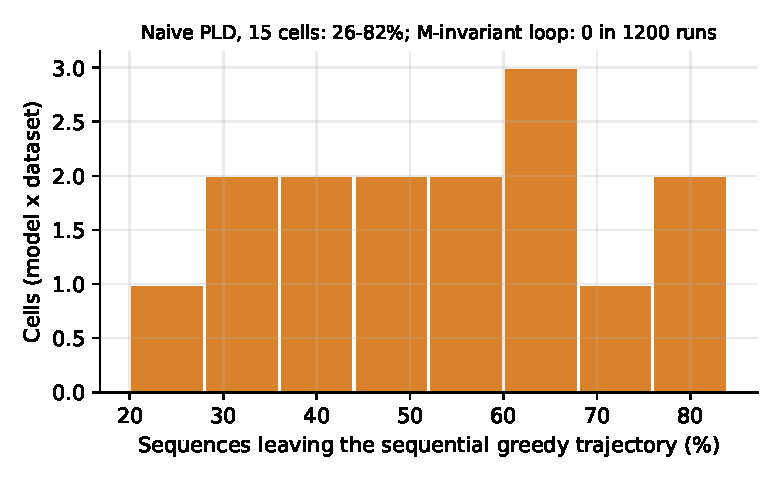
\includegraphics[width=0.6\textwidth]{images/kernel_naive_divergence.pdf}
\caption{Phân bố tỷ lệ chuỗi lệch quỹ đạo greedy tuần tự của PLD ngây thơ trên 15 ô (mô hình $\times$ tập dữ liệu).}\label{fig:k-naive}
\end{figure}

\section{Định nghĩa exact và tham chiếu}\label{sec:k-ref}
Gọi $\mathcal K$ là một bộ kernel cố định và $R_{\mathcal K}$ là giải mã greedy tuần tự dùng $\mathcal K$ với $M{=}1$ ở mọi bước. Một bộ giải mã suy đoán là \emph{exact theo $\mathcal K$} nếu với mọi prompt nó trả về đúng các token của $R_{\mathcal K}$ và để lại đúng các byte KV cache của $R_{\mathcal K}$. Ta \emph{không} đòi bằng greedy bitsandbytes gốc: đó là một bộ kernel khác.

Hai bộ kernel hợp lệ khác thứ tự cộng thì tách nhau. Phép đo trên Qwen2.5-3B (\cref{tab:k-ref}) cho thấy chuỗi từ tham chiếu bất biến giống hệt chuỗi bitsandbytes gốc ở chỉ $30\%$ ($n{=}50$) và $44\%$ ($n{=}150$) số prompt GSM8K, cùng cỡ với mức lệch của PLD ngây thơ. Độ chính xác tác vụ không bị phát hiện giảm: GSM8K $72\%$ so với $66\%$ ($n{=}50$, $5$ so với $2$ cặp bất đồng, trong nhiễu). Đây là kiểm tra không phát hiện sai khác, không phải chứng minh tương đương. Trên HumanEval ($n{=}100$, prompt thô, tối đa $384$ token) pass@1 là $61/100$ ở cả hai chế độ, với $3$ và $3$ bài bất đồng theo hai chiều; chuỗi token giống hệt ở $72/100$ prompt (mức giống cao hơn GSM8K vì đầu ra ngắn hơn). Con số $61\%$ thấp hơn mức công bố cho mô hình vì ta dùng prompt thô và cắt hoàn thành bằng quy tắc đơn giản, nên chỉ có ý nghĩa để so hai chế độ với nhau.

\begin{table}[t]
\centering\small
\caption{Tham chiếu bất biến so với greedy bitsandbytes gốc, Qwen2.5-3B NF4.}\label{tab:k-ref}
\begin{tabular}{@{}lrrr@{}}
\toprule
Phép đo & $n$ & Gốc & Bất biến\\\midrule
Chuỗi giống hệt (GSM8K) & 50 & \multicolumn{2}{c}{$15$ ($30\%$)}\\
Chuỗi giống hệt (GSM8K, ext150) & 150 & \multicolumn{2}{c}{$66$ ($44\%$)}\\
Độ chính xác GSM8K & 50 & $33$ ($66\%$) & $36$ ($72\%$)\\
Chuỗi giống hệt (HumanEval) & 100 & \multicolumn{2}{c}{$72$ ($72\%$)}\\
pass@1 HumanEval & 100 & $61$ ($61\%$) & $61$ ($61\%$)\\
\bottomrule
\end{tabular}
\end{table}

\section{Thiết kế kernel bất biến}\label{sec:k-design}
\paragraph{Nguyên tắc.} Phần tử đầu ra $(m,n)$ được tính bởi cùng một dãy lệnh bất kể $M$ và các hàng khác. Có bốn quy tắc: (i) đệm số 0 khối hàng về kích thước cố định $M_P$; (ii) thứ tự rút gọn theo $K$ cố định; (iii) không split-K, không atomics, không tự điều chỉnh (autotune); (iv) không có phụ thuộc dữ liệu giữa các hàng. Bất biến được kiểm bằng thực nghiệm (hàng chục nghìn hàng mỗi kernel); chương này không chứng minh hình thức. \cref{fig:k-principle} minh họa nguyên tắc.


\begin{figure}[t]
\centering
\begin{tikzpicture}[x=1cm,y=1cm,font=\small]
  % input rows
  \foreach \i/\lab in {0/$x_0$,1/$x_1$,2/$x_2$} { \draw[fill=blue!15] (0,-\i*0.6) rectangle (2.4,-\i*0.6-0.5); \node at (1.2,-\i*0.6-0.25) {\lab}; }
  \foreach \i in {3,4,5} { \draw[dashed,fill=gray!10] (0,-\i*0.6) rectangle (2.4,-\i*0.6-0.5); \node at (1.2,-\i*0.6-0.25) {0}; }
  \node[align=center] at (1.2,0.45) {khối $M{=}3$ hàng\\đệm $0$ tới $M_P$};
  \draw[->,thick] (2.6,-1.5) -- (3.6,-1.5);
  % kernel
  \draw[fill=orange!15] (3.7,-3.2) rectangle (7.7,0.3);
  \node[align=center] at (5.7,-0.4) {\textbf{kernel bất biến}};
  \node[align=left,font=\footnotesize] at (5.7,-1.8) {thứ tự rút gọn $K$ cố định\\không split-K / atomics\\không autotune\\mỗi hàng độc lập};
  \draw[->,thick] (7.9,-1.5) -- (8.9,-1.5);
  % outputs
  \foreach \i/\lab in {0/$y_0$,1/$y_1$,2/$y_2$} { \draw[fill=green!15] (9.0,-\i*0.6) rectangle (11.4,-\i*0.6-0.5); \node at (10.2,-\i*0.6-0.25) {\lab}; }
  \node[align=center,font=\footnotesize] at (10.2,-2.4) {$y_i$ giống từng bit\\với chạy $M{=}1$};
\end{tikzpicture}
\caption{Nguyên tắc thiết kế: khối $M$ hàng được đệm $0$ tới kích thước cố định $M_P$ và đi qua cùng một dãy lệnh; kết quả mỗi hàng không phụ thuộc $M$.}\label{fig:k-principle}
\end{figure}

\paragraph{LM head.} Kernel Triton dùng \code{tl.dot} trên khối $16$ hàng (đệm $0$), fp16/bf16 $\to$ fp32, $K$ chia khối $128$ theo thứ tự cố định. Kết quả bằng từng bit với GEMM cuBLAS khi $M{\ge}2$ nhưng không bằng đường gemv của cuBLAS ở $M{=}1$ ($1.2\%$ phần tử khác); đây là lý do tham chiếu không trùng bitsandbytes gốc. Chi phí $3.42$~ms so với $3.34$~ms của cuBLAS ở $M{=}1$ ($1.02\times$) và gần như không đổi theo $M{=}1..8$; chạy từng hàng ba lần tốn $10.8$~ms.

\paragraph{Attention.} Kernel Triton split-KV với các đoạn khóa tuyệt đối (256 khóa, tile 64): mỗi đoạn tính softmax trực tuyến riêng, các kết quả riêng được gộp theo thứ tự đoạn tăng dần. Đoạn bị che hoàn toàn là phép không (no-op) chính xác, nên kết quả một hàng không phụ thuộc vào số hàng hay vị trí sau nó. Ở chế độ CUDA graph, độ dài tiền tố là một số \code{int32} trên thiết bị. GQA dùng K/V gọn. Ở $M{=}3$ nhanh hơn SDPA có mặt nạ $5$--$25$ lần.

\paragraph{RMSNorm.} Mỗi chương trình xử lý đúng một hàng.

\paragraph{GEMM NF4.} Kernel CUDA C++ dùng bố cục bitsandbytes (nibble cao trước, blocksize $64$, absmax lượng tử hóa kép). Một warp xử lý $R$ hàng đầu ra và $M_P$ hàng kích hoạt; trọng số được đọc và giải lượng tử một lần cho mọi hàng, đây là nơi có lợi ích so với chạy từng hàng. Mỗi lane xử lý $32$ phần tử $K$ mỗi bước $1024$ phần tử, cộng dồn \code{fmaf} theo thứ tự cố định rồi rút gọn xor-butterfly. Các biến thể $M_P\in\{1,2,4,8\}$ và $R\in\{1,2,4,8\}$ cho cùng từng bit trên mỗi hàng ($0$ lệch trên $7000$ hàng). Hai phiên bản Triton đầu chậm hơn bitsandbytes $4$--$20$ lần nên bị bỏ.

\begin{algorithm}[t]
\caption{Kernel GEMM NF4 bất biến theo $M$ (một warp).}\label{alg:nf4}
\begin{algorithmic}[1]
\Require $R$ hàng trọng số NF4, $M\le M_P$ hàng kích hoạt (đệm $0$ tới $M_P$)
\Ensure $Y[m,r]$ với $m<M$, độ lớn không phụ thuộc $M$
\For{$k_0 = 0,1024,2048,\dots$} \Comment{thứ tự cố định}
  \State mỗi lane nạp $32$ nibble của mỗi hàng trọng số, giải lượng tử một lần
  \For{$m=0..M_P-1$, $r=0..R-1$}
    \State $acc[m,r] \gets \mathrm{fmaf}(x[m,k], w[r,k], acc[m,r])$ theo $k$ tăng dần
  \EndFor
\EndFor
\State rút gọn $acc[m,r]$ qua $32$ lane bằng xor-butterfly cố định
\State cộng bias (fp32) và làm tròn về dtype đầu ra
\end{algorithmic}
\end{algorithm}

\paragraph{Một lỗi mà kiểm tra ``exact'' không bắt được.} Bản đầu của kernel NF4 đọc bias fp16 như bf16 và cho đầu ra vô nghĩa trong mô hình thật, nhưng vẫn ``exact'' $100\%$ vì mọi cách chạy đều sinh cùng một chuỗi lặp vô nghĩa. Lỗi chỉ lộ khi đọc văn bản sinh ra; đã sửa (bias chuyển sang fp32) và so từng lớp với ma trận giải lượng tử fp32 trên kích hoạt thật. Bài học: kiểm tra exact phải đi kèm kiểm tra văn bản hoặc độ chính xác tác vụ. Mọi số liệu tốc độ trong chương đều sinh sau bản sửa.

\begin{table}[t]
\centering\small
\caption{Kiểm chứng bất biến theo $M$ (số hàng lệch / tổng số hàng kiểm).}\label{tab:k-inv}
\begin{tabular}{@{}lrl@{}}
\toprule
Kernel & Hàng kiểm & Lệch\\\midrule
LM head (5 hình dạng) & 27\,000 & 0\\
Attention (Qwen 3B, 1.5B, 0.5B; ngữ cảnh $128$--$3000$) & $3\times 6300$ & 0\\
Attention MHA $32/32$ & 2\,100 & 0\\
GEMM NF4 (mọi biến thể $M_P$, $R$) & 7\,000 & 0\\
\bottomrule
\end{tabular}
\end{table}

\section{Chi phí một bước giải mã}\label{sec:k-cost}
Thời gian một bước giải mã đầy đủ trong CUDA graph (Qwen2.5-3B): $M{=}1$ $15.0$~ms (bitsandbytes $16.3$), $M{=}3$--$4$ $17.7$~ms (bitsandbytes $21.2$ đến $31.5$), $M{=}5$--$6$ $23.6$~ms (bitsandbytes $31$) (\cref{fig:k-step}). Kernel GEMM chiếm $9.2$~ms ở $M{=}1$, chậm hơn \code{gemm_4bit_simt} của bitsandbytes ($8.9$~ms) khoảng $3\%$ nhưng nhanh rõ ở $M{\ge}3$. Nghĩa là bước kiểm tra $M{=}3$ chỉ đắt hơn bước $M{=}1$ khoảng $18\%$, đúng điều kiện để giải mã suy đoán có lợi.

\begin{figure}[t]
\centering
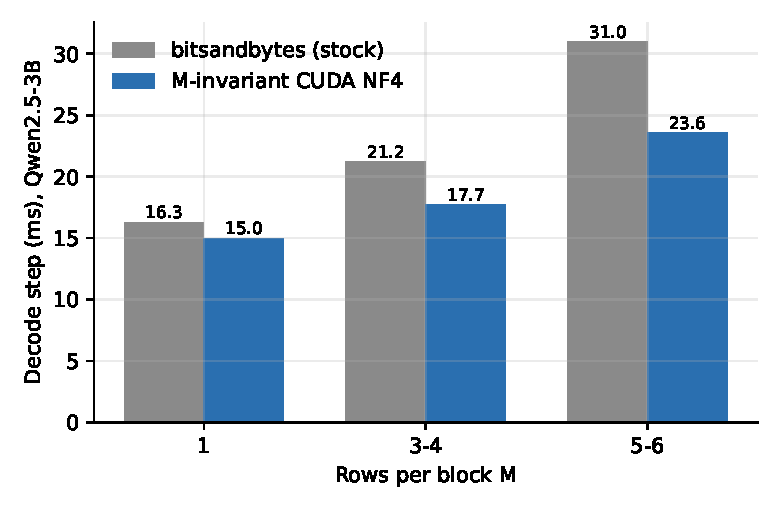
\includegraphics[width=0.55\textwidth]{images/kernel_step_time.pdf}
\caption{Thời gian một bước giải mã trong CUDA graph, Qwen2.5-3B NF4, theo số hàng của khối.}\label{fig:k-step}
\end{figure}

\section{Vòng giải mã exact trên CUDA graph}\label{sec:k-loop}
PLD đề xuất tối đa $K{=}2$ token (n-gram $3$); khối $M\le 3$ hàng được kiểm tra bằng các kernel bất biến trong một lần phát lại CUDA graph; token được chấp nhận được commit, hàng bị loại được quay lui bằng cách đặt lại độ dài của static cache (\code{cumulative_length.fill_(n)}); tensor tiền tố của attention được cập nhật trước mỗi lần phát lại. Vì mọi kernel bất biến theo $M$, byte KV đã commit bằng của giải mã tuần tự, điều ta kiểm trực tiếp.

\begin{algorithm}[t]
\caption{Vòng PLD exact với kernel bất biến.}\label{alg:loop}
\begin{algorithmic}[1]
\Require prompt, tham chiếu $R_{\mathcal K}$, $K{=}2$
\State prefill bằng kernel bất biến; $n \gets$ độ dài tiền tố
\While{chưa EOS và chưa đủ token}
  \State $d \gets$ tra n-gram (tối đa $K$ token) \Comment{có thể rỗng}
  \State chạy khối $1{+}|d|$ hàng bằng đồ thị CUDA ($M\in\{1,2,3\}$)
  \State $j \gets$ số token nháp khớp argmax; commit $j{+}1$ token
  \State \code{cumulative_length.fill_(n + j + 1)}; $n \gets n+j+1$ \Comment{quay lui KV}
\EndWhile
\end{algorithmic}
\end{algorithm}

\section{Kết quả đầu-cuối}\label{sec:k-results}
\paragraph{Thiết lập.} RTX 4050 Laptop 6~GB, Triton 3.6.0, nvcc 12.8, bitsandbytes 0.50.0, greedy, batch 1, $128$ token mới, $K{=}2$, n-gram $3$. Baseline là giải mã $M{=}1$ exact dùng cùng kernel bất biến trong CUDA graph, cùng phiên và cùng prompt. ``Exact'' là token sinh ra \emph{và} KV đã commit bằng từng bit với $R_{\mathcal K}$.

\begin{table}[t]
\centering\small
\caption{Vòng PLD exact so với baseline $M{=}1$ cùng kernel. Tăng tốc theo prompt là trung vị [min, max]. Cận trên Wilson $95\%$ của tỷ lệ lệch: $1.9\%$ ($n{=}200$), $3.7\%$ ($n{=}100$).}\label{tab:k-speed}
\begin{tabular}{@{}lrrrrrl@{}}
\toprule
Ô & Prompt & Exact & Base & PLD & Tăng & Theo prompt\\\midrule
Qwen2.5-3B GSM8K & 200 & 200/200 & 61.2 & 71.8 & $1.17\times$ & $1.18$ [1.01, 1.40]\\
Qwen2.5-3B HumanEval & 100 & 100/100 & 58.9 & 77.6 & $1.32\times$ & $1.32$ [1.01, 2.22]\\
Qwen2.5-3B CNN/DM & 100 & 100/100 & 58.7 & 70.7 & $1.21\times$ & $1.21$ [0.98, 1.54]\\
Qwen2.5-1.5B GSM8K & 100 & 100/100 & 97.1 & 115.6 & $1.19\times$ & $1.18$ [1.01, 1.53]\\
Qwen2.5-0.5B GSM8K & 100 & 100/100 & 196.0 & 241.9 & $1.23\times$ & $1.22$ [1.05, 1.67]\\
OLMo-2-1B GSM8K & 100 & 100/100 & 136.2 & 155.1 & $1.14\times$ & $1.13$ [1.02, 1.37]\\
Phi-3.5-mini GSM8K & 100 & 100/100 & 72.7 & 85.9 & $1.18\times$ & $1.18$ [1.05, 1.41]\\
Llama-3.2-1B GSM8K & 100 & 100/100 & 135.1 & 171.5 & $1.27\times$ & $1.26$ [1.04, 2.15]\\
Llama-3.2-3B GSM8K & 100 & 100/100 & 62.9 & 78.2 & $1.24\times$ & $1.21$ [1.05, 2.20]\\
Mistral-7B GSM8K & 100 & 100/100 & 38.1 & 45.8 & $1.20\times$ & $1.20$ [1.07, 1.50]\\
Mistral-7B HumanEval & 100 & 100/100 & 35.5 & 44.1 & $1.24\times$ & $1.21$ [1.00, 1.94]\\
\bottomrule
\end{tabular}
\end{table}

Tổng cộng $1200$ cặp (prompt, mô hình) trên $8$ mô hình (năm họ Qwen2.5, OLMo-2, Phi-3.5, Llama-3.2 và Mistral; GQA và MHA; $head\_dim$ $64$, $96$ và $128$): $0$ lệch về token và KV; các lần chạy lặp (cùng phiên so sánh, kiểm tra EOS, kiểm tra phiên bản) cũng đều exact. Tăng tốc $1.14$--$1.32\times$; chỉ một prompt (CNN/DM) chậm hơn baseline ($0.98\times$) (\cref{fig:k-cells}). Phi-3.5 cần hai chỉnh sửa hạ tầng chứ không đổi kernel: kernel attention được mở rộng cho $head\_dim$ $96$ (đệm lên $128$ trong kernel bằng mặt nạ, $0$ lệch trên $700$ hàng, bốn kernel cũ vẫn $0$ lệch), RoPE LongRoPE được cố định ở chế độ hệ số ngắn (đúng với ngữ cảnh dưới $4096$ token, vì bản gốc chọn hệ số bằng một phép đồng bộ dữ liệu làm hỏng CUDA graph), và cache dùng lớp tĩnh thông thường thay cho lớp cửa sổ trượt (cửa sổ $262144$ lớn hơn ngữ cảnh, lớp cửa sổ trượt giữ độ dài bằng số nguyên Python nên không quay lui được). Lần chạy đầu của Phi-3.5 trước khi sửa lớp cache cho tốc độ cao bất thường ($1.74\times$) nhưng không exact; cờ exact đã phát hiện được lỗi này. Hai mô hình Llama-3.2 và Mistral-7B-Instruct-v0.3 (bản sao không cần token của unsloth; Mistral là mô hình $7$B đầu tiên, tải sẵn dạng NF4 và vừa GPU $6$~GB với cache ngắn) chạy không cần sửa gì. Trên Mistral-7B, một bước giải mã $M{=}1$ tốn khoảng $26$--$28$~ms, gần gấp đôi mô hình $3$B, nhưng mức tăng của PLD ($1.20$--$1.24\times$) tương đương các mô hình nhỏ; ở HumanEval, tăng tốc chỉ trên $55$ prompt không có EOS là $1.28\times$. Baseline $M{=}1$ bất biến còn nhanh hơn baseline graph kernel gốc ($62.4$ so với $57.8$~tok/s trên GSM8K).

\begin{figure}[t]
\centering
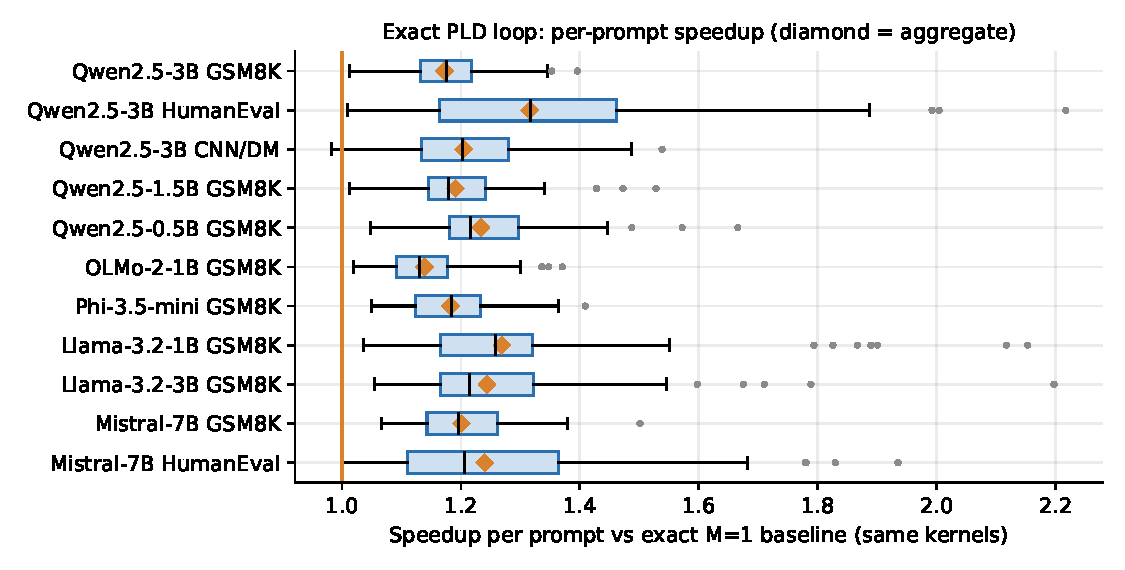
\includegraphics[width=0.85\textwidth]{images/kernel_speedup_cells.pdf}
\caption{Phân bố tăng tốc theo prompt của vòng PLD exact so với baseline $M{=}1$ cùng kernel.}\label{fig:k-cells}
\end{figure}

\paragraph{So với vòng exact cũ chạy từng hàng.} Cùng prompt, chạy liền nhau (vòng cũ, vòng mới, vòng cũ để đo trôi): với $100$ prompt mỗi tập, vòng mới đạt $79.0$ tok/s trên GSM8K so với $62.7$ và $61.2$ của vòng cũ ($1.26\times$ và $1.29\times$), $76.5$ so với $56.4$ và $57.0$ trên CNN/DM ($1.36\times$ và $1.34\times$), $81.9$ so với $58.9$ và $59.4$ trên HumanEval ($1.39\times$ và $1.38\times$); tất cả các lượt đều exact. Hai lần chạy vòng cũ lệch nhau nhiều nhất $2.4\%$, nên nhiễu giữa các phiên nhỏ hơn mức chênh. So với baseline $M{=}1$ bất biến cùng phiên, mức tăng trong các phiên này là $1.18\times$, $1.20\times$ và $1.31\times$ (nhanh hơn một chút so với Bảng~\ref{tab:k-speed} do phiên chạy khác nhau).

\paragraph{Ablation.} PLD với $K{=}4$ chậm hơn $K{=}2$ ($1.145\times$ so với $1.206\times$, 10 prompt). Tắt làm tròn trọng số hay thay tra bảng bằng phép tính chỉ đổi thời gian GEMM dưới $5\%$; ở $M{=}4$ kernel gần giới hạn số phép FMA, ở $M{=}1$ còn cách giới hạn băng thông khoảng $20\%$. Ước tính tối đa $10\%$ thời gian bước còn thu hồi được, tăng đều cho cả baseline lẫn vòng PLD nên gần như không đổi tỷ số tăng tốc.

\paragraph{Kiểm tra văn bản sau EOS.} Vòng sinh đúng $128$ token và không dừng ở EOS, nên với prompt có EOS sớm phần sau là văn bản lặp, thứ mà PLD đoán rất dễ và có thể làm tăng tốc cao hơn thực tế. Ta chạy lại sáu ô (100 prompt mỗi ô) ghi vị trí EOS đầu tiên của chuỗi tham chiếu: tỷ lệ prompt có EOS trong $128$ token là $0\%$ (Qwen-3B GSM8K), $26\%$ (HumanEval), $8\%$ (CNN/DM), $9\%$ (Llama-3B), $17\%$ (Llama-1B) và $15\%$ (Phi-3.5). Tăng tốc chỉ tính trên các prompt không có EOS lần lượt là $1.18$, $1.32$, $1.21$, $1.23$, $1.29$ và $1.19\times$, so với $1.18$, $1.32$, $1.20$, $1.24$, $1.27$ và $1.18\times$ khi tính mọi prompt (lệch dưới $2\%$); cả $600$ lượt chạy này đều exact. Văn bản sau EOS vì vậy không làm tăng số đo.

\section{Độ phụ thuộc vào phiên bản bitsandbytes}\label{sec:k-bnbver}
Kernel GEMM NF4 của ta chỉ dùng bố cục lượng tử hóa của bitsandbytes, không gọi kernel nhân của nó, nên bộ kernel không phụ thuộc cách bitsandbytes chọn kernel. Ngược lại, hành vi của đường gốc mà ta thay thế phụ thuộc phiên bản. Ta đo tỷ lệ phần tử khác từng bit giữa phép chiếu NF4 chạy cả khối $M$ hàng và chạy từng hàng, trên dữ liệu ngẫu nhiên với ba hình dạng của Qwen2.5-3B (\cref{tab:k-bnbver}): bitsandbytes 0.50.0 và 0.50.1 cho kết quả giống hệt nhau (ổn định đến $M{=}3$ và lệch $\approx60\%$ phần tử từ $M{\ge}4$), còn 0.49.2 (trước PR \#1949 thêm kernel GEMM 4-bit hợp nhất) lệch $\approx60\%$ ngay từ $M{=}2$. Nói cách khác ngưỡng $M{=}4$ chỉ là tính chất của 0.50.x; trên 0.49.2 ngay cả khối hai hàng cũng không an toàn. Bộ kernel bất biến vượt cả bốn kiểm tra đơn vị và vòng exact trên 20 prompt GSM8K với cả 0.49.2 và 0.50.1 ($20/20$ exact, tăng $1.19\times$ và $1.20\times$ so với baseline $M{=}1$ bất biến). Các tỷ lệ $\approx60\%$ lớn hơn $13$--$15\%$ ở Bảng~\ref{tab:k-audit} vì dữ liệu ngẫu nhiên fp16 khác kích hoạt thật; chỉ so sánh giữa các phiên bản mới có ý nghĩa.

\begin{table}[t]
\centering\small
\caption{Tỷ lệ phần tử NF4 khác từng bit giữa khối $M$ hàng và chạy từng hàng (stock bitsandbytes, hình dạng $11008{\times}2048$, dữ liệu ngẫu nhiên).}\label{tab:k-bnbver}
\begin{tabular}{@{}lrrrrr@{}}
\toprule
Phiên bản & $M{=}2$ & $M{=}3$ & $M{=}4$ & $M{=}8$ & $M{=}16$\\\midrule
0.49.2 & 60.5\% & 60.2\% & 60.2\% & 60.3\% & 60.4\%\\
0.50.0 & 0\% & 0\% & 60.2\% & 60.3\% & 60.4\%\\
0.50.1 & 0\% & 0\% & 60.2\% & 60.3\% & 60.4\%\\
\bottomrule
\end{tabular}
\end{table}

\section{Kết quả âm}\label{sec:k-neg}
\begin{itemize}[nosep]
\item \textbf{Mô hình nháp thần kinh.} Qwen2.5-0.5B bf16 nháp cho 3B NF4 ($K{=}2$) exact nhưng chỉ $0.66\times$ baseline: một bước nháp tốn khoảng $10$~ms so với $15$~ms của một bước đích. Tính từ số đo, ngay cả nháp nén NF4 cũng chỉ khoảng $0.87\times$, và nháp miễn phí bị chặn ở khoảng $1.36\times$. Với đích 4-bit $3$B đã rất rẻ trên GPU này, PLD là nguồn nháp phù hợp. Với đích $\ge7$B tình hình có thể khác nhưng chưa đo được.
\item \textbf{Tối ưu kernel} còn tối đa khoảng $10\%$ (mục trước).
\item Tiêu chí ban đầu ``$\ge1.15\times$ với mô hình nháp thật'' \emph{không đạt}; chỉ PLD đạt tăng tốc.
\end{itemize}

\section{Giới hạn và mối đe dọa tính hợp lệ}\label{sec:k-limits}
(i) Một GPU (RTX 4050 6~GB), mô hình tới $7$B (chỉ một mô hình $7$B, với cache ngắn), batch $1$, chỉ greedy; chưa chạy mô hình $\ge7$B hay GPU khác. (ii) Bất biến dựa vào cấu trúc kernel và thực nghiệm, không phải chứng minh, và phụ thuộc phiên bản trình biên dịch (Triton 3.6.0, nvcc 12.8); các kiểm tra bất biến và vòng exact (20 prompt) cũng đạt với bitsandbytes 0.49.2 và 0.50.1 (xem mục~\ref{sec:k-bnbver}), nhưng chỉ trên một GPU. (iii) Chưa thử họ kiến trúc nào ngoài Qwen2, OLMo-2, Phi-3 và Llama-3.2 (chưa có Gemma và mô hình MoE). (iv) Tăng tốc phụ thuộc mức PLD tìm được bản nháp: cao nhất ở HumanEval, thấp nhất ở OLMo-2. (v) So sánh độ chính xác với tham chiếu gốc còn nhỏ ($n{=}50$ trên GSM8K). (vi) Phi-3.5 chỉ được hỗ trợ trong chế độ ngữ cảnh $\le4096$ token (hệ số LongRoPE ngắn). (vii) Mọi prompt dùng văn bản thô (không dùng chat template). (viii) So sánh với LLM-42 và các công trình đồng thời mới ở mức đọc tài liệu.

\section{Tóm tắt chương}
Bộ kernel bất biến theo $M$ (LM head, attention, RMSNorm, GEMM NF4) cho phép kiểm tra theo khối exact theo bộ kernel của chính nó, và vòng PLD trên CUDA graph chạy nhanh hơn giải mã exact $M{=}1$ cùng kernel $1.14$--$1.32\times$ với $0$ lệch trong $1200$ cặp prompt-mô hình. Mức tăng là khiêm tốn, phụ thuộc workload và chỉ có với PLD; mô hình nháp thần kinh không có lợi trên đích $3$B. Tham chiếu exact là bộ kernel mới, khác bitsandbytes gốc ở phần lớn chuỗi nhưng không phát hiện giảm độ chính xác tác vụ ở cỡ mẫu nhỏ.

\paragraph{Mã nguồn.} \texttt{src/zassd/kernels/}, \texttt{scripts/wp*}, số liệu ở \texttt{results/kernels/}; kế hoạch và bản thảo bài báo ở \texttt{docs/PLAN\_SHAPE\_INVARIANT\_KERNELS.md} và \texttt{docs/PAPER\_DRAFT\_KERNELS.md}.

\clearpage
\chapter{Kết luận và hướng phát triển}

\section{Kết luận}

Đồ án đã xây dựng và khảo sát ZASSD, một hệ thống giải mã suy đoán không cần nạp checkpoint draft độc lập. Hệ thống gồm đường vanilla, Prompt Lookup Decoding (PLD), self-speculation bằng layer-skip, bộ định tuyến kết hợp các hành động, target verification và quản lý KV cache. Các phép đo được tổ chức theo cohort riêng để phân biệt kết quả hiệu năng, numerical fidelity và chẩn đoán kernel.

Trong benchmark paired 150 prompt trên Qwen2.5-3B-Instruct NF4, PLD đạt speedup end-to-end trung bình paired \(1.063\times\) so với vanilla (CI bootstrap 95\%: \([1.036,1.092]\)); router đạt \(1.050\times\), nhưng chậm hơn PLD theo tỷ số paired \(0.989\) (CI: \([0.985,0.993]\)). Kết quả cho thấy PLD có thể tăng throughput trong cấu hình đã thử, còn router chưa chứng minh lợi ích so với baseline cố định mạnh nhất. Exact sequence match 83.3\% cũng cho thấy speedup không đồng nghĩa với bảo toàn hoàn toàn chuỗi đầu ra.

Các phân tích bổ sung cho thấy chi phí cycle, backend và cách tổ chức verification đều liên quan đến hiệu năng và fidelity. Tuy nhiên, cohort chẩn đoán được chọn có chủ đích, phép profiling chỉ chạy trên một prompt, và verification tuần tự chỉ khôi phục sequence identity trong các mẫu đã kiểm tra. Vì vậy, đóng góp chính của đồ án là một hệ thống có thể so sánh các đường giải mã trong cùng framework cùng một đánh giá thực nghiệm có giới hạn rõ ràng; kết quả chưa bảo đảm khả năng khái quát sang cấu hình khác.

Chương 6 mở rộng phần đánh giá sang tính exact: một vòng giải mã suy đoán B2 trên NF4 tái tạo đúng từng token và KV của greedy bitsandbytes gốc ở mọi prompt đã kiểm, gồm hai cohort held-out GSM8K mỗi cohort 50 prompt dùng đúng một lần (khớp $50/50$ ở cả hai), không dùng thêm bộ nhớ đáng kể ($0.07$~MiB ở đỉnh) và nhanh hơn bitsandbytes eager khoảng $1.12$--$1.15\times$. Mức tăng này khiêm tốn và bị giới hạn bởi chi phí khởi chạy kernel của CPU và acceptance của PLD; B2 chậm hơn một baseline \texttt{torch.compile} (khoảng $0.91\times$ tốc độ của nó) vốn không exact, nên đóng góp nằm ở tính exact và quy trình bằng chứng chứ không ở tốc độ tuyệt đối.

Chương 7 đi tiếp từ giới hạn tốc độ của B2: bộ kernel 4-bit bất biến theo số hàng (LM head, attention, RMSNorm, GEMM NF4) cho phép kiểm tra theo khối mà vẫn exact theo bộ kernel của chính nó. Vòng PLD exact trên CUDA graph cho $0$ lệch token và KV trên $1200$ cặp prompt-mô hình, tám mô hình và ba tập dữ liệu, nhanh hơn baseline exact $M{=}1$ cùng kernel $1.14$--$1.32\times$ và nhanh hơn vòng B2 chạy từng hàng khoảng $1.26$--$1.39\times$. Cái giá là tham chiếu exact khác bitsandbytes gốc ở phần lớn chuỗi (chỉ $30$--$44\%$ giống hệt), dù không phát hiện giảm độ chính xác tác vụ ở cỡ mẫu nhỏ; và mô hình nháp thần kinh không có lợi trên đích $3$B ($0.66\times$). Đóng góp nằm ở bộ kernel, định nghĩa exact theo bộ kernel và quy trình bằng chứng, không ở tốc độ tuyệt đối.

\section{Hạn chế}

Kết quả benchmark chính được thu trên một NVIDIA RTX 4050 Laptop GPU, một mô hình Qwen2.5-3B-Instruct, NF4/FP16 compute và SDPA. Số prompt benchmark chính là 150, nhưng các cohort router, numerical fidelity và profiling nhỏ hơn và dùng giao thức khác. Nhiệt độ GPU thay đổi trong các snapshot của benchmark; dù thứ tự phương pháp được xoay vòng, phép đo một thiết bị vẫn có thể chịu ảnh hưởng nhiệt và trạng thái hệ thống.

Một số nhóm numerical fidelity được chọn có chủ đích từ các prompt đã có mismatch trước đó; tỷ lệ đúng/sai ở nhóm này phục vụ chẩn đoán, không ước lượng tỷ lệ lỗi trong traffic tự nhiên. Cohort held-out 14 prompt thuộc cùng prepared-input artifact, không phải đánh giá ngoài độc lập. Phép Nsight có instrumentation và chỉ bao phủ một prompt, còn các thống kê cycle gộp không lưu số candidate draft cho từng cycle. Chưa có đủ bằng chứng để khái quát sang GPU, model, quantization, attention backend hoặc workload khác.

Đối với Chương 6, bằng chứng đều từ một GPU và một bộ công cụ (bitsandbytes 0.50.0, Triton 3.6.0, PyTorch 2.11.0), chủ yếu một họ mô hình (Qwen2) và một backend lượng tử hóa, batch 1, greedy. Tính exact dựa trên bằng chứng hữu hạn chứ chưa phải chứng minh: còn mở sự bằng nhau với kernel bitsandbytes trên mọi đầu vào (mã nguồn CUDA đọc theo nghĩa đen khác với hành vi của bản nhị phân), độc lập của dispatch PyTorch với số hàng, độ ổn định qua phiên bản Triton/ptxas/CUDA và GPU, và kiểm ở mức PTX.

Cuối cùng, exact match với greedy vanilla chỉ đo đồng nhất token ID trong cùng cấu hình. Nó không thay thế đánh giá chất lượng tác vụ, và numerical equivalence của KV/logits cũng không thể được suy ra chỉ từ việc chuỗi đầu ra giống nhau. Các phép đo bộ nhớ dùng peak allocated memory của PyTorch trong một cohort riêng; chúng không đại diện cho toàn bộ VRAM do driver/NVML báo cáo.

\section{Hướng phát triển}

Các công việc tiếp theo được ưu tiên như sau:
\begin{enumerate}
    \item Mở rộng benchmark paired sang nhiều GPU, model và backend; lặp phiên chạy độc lập để định lượng biến thiên giữa phiên, nhiệt độ và thứ tự chạy.
    \item Bổ sung số liệu theo cycle: candidates, accepted/emitted tokens, thời gian không chồng lấn và action fallback. Dùng chúng để kiểm định cost model độc lập.
    \item Cải thiện router bằng baseline PLD mạnh đã hiệu chỉnh trên tập development, sau đó đánh giá trên held-out traffic; báo cáo riêng lựa chọn action, overhead, speedup và fidelity.
    \item Tiếp tục phân tích sai khác số học giữa batched và sequential verification, KV history, NF4 và các backend khác; thiết kế chế độ fallback có thể bảo toàn sequence identity với overhead được đo rõ.
    \item Đo thêm chất lượng tác vụ, latency đầu-cuối, VRAM allocated/reserved/NVML và prompt/đầu ra đa dạng.
    \item Chạy bộ kernel bất biến trên GPU khác và mô hình $\ge7$B (nơi mô hình nháp thần kinh có thể có lợi), thử bitsandbytes 0.50.1/0.50.2, hỗ trợ $head\_dim$ $96$ (Phi-3.5), và chứng minh hình thức hoặc kiểm ở mức PTX tính bất biến.
    \item Kiểm tra vòng giải mã exact B2 trên GPU và phiên bản Triton/bitsandbytes khác, ở mức PTX, trên backend lượng tử hóa và họ mô hình khác, và hoàn thiện lập luận theo toán tử; mọi lần nâng cấp bitsandbytes cần chạy lại phép mô phỏng thứ tự rút gọn của kernel.
\end{enumerate}

Mục tiêu là xác định được miền cấu hình mà lợi ích throughput của speculative decoding đủ lớn, có thể tái lập và đáp ứng ngưỡng chính xác của ứng dụng, thay vì giả định một phương pháp duy nhất luôn tốt nhất.

\clearpage

\renewcommand{\bibname}{Tài liệu tham khảo}
\addcontentsline{toc}{chapter}{Tài liệu tham khảo}
\bibliographystyle{unsrt}
\bibliography{references}

\end{document}
